\documentclass{article}
\usepackage{fancyhdr}
\usepackage{graphicx}
\usepackage{amsmath}
\usepackage{xcolor}
\usepackage{caption}
%\usepackage{hyperref}
\usepackage[margin=1in]{geometry}

\pagestyle{fancy}
\graphicspath{ {./img/} }

\begin{document}
	\begin{titlepage}
		\begin{center}
			\vspace{1cm}
			{\LARGE\textbf{The Bipolar Junction Transistor (BJT): DC and AC Characterization}}

			\vspace{1.5cm}
			\textbf{\large Ghassan Arnouk}\\
			
			\vspace{1cm}
			\large ELEC 3509B\\
			\large Summer 2020\\
			\large Lab 1 Report\\
			
						
			\vspace{2cm}
			\textbf{Instructor:} Qi-Jun Zhang\\
						
			
			\vspace{1cm}
			\textbf{Lab Period:} B1\\
			
			\vspace{0.1cm}
			\textbf{Day 1 Preformed:} 2020/07/09
			
			\vspace{0.1cm}
			\textbf{Day 2 Preformed:} 2020/07/15
			
			\vspace{1cm}
			\textbf{Date Submitted:} 2020/07/22\\			
		\end{center}
	\end{titlepage}

	\lhead{Ghassan Arnouk (B1)}
	\rhead{BJT: DC and AC Characterization}
	\pagebreak
	
	\tableofcontents
	\pagebreak
		
	\listoftables
	\pagebreak
	
	\listoffigures
	\pagebreak
	
	\section{Introduction}
	\subsection{Purpose}
	The purpose of this lab is to explore the device characterization of a Bipolar Junction Transistor (BJT).
	This process helps to obtain important device parameters which allows the designer to obtain information that the datasheet might not have and compare the results.
	
	\subsection{Experiment Overview}
	In day 1, the DC characterization of the transistor was analyzed.
	Data were measured and the I-V curves of the transistor were generated.
	As well, a current mirror circuit was assembled and tested which has given an idea of the way they work and where their limitations are.\\\\
	In day 2, the AC characterization of the transistor was analyzed.
	Data were obtained with performing medium and higher frequency measurements.
	Then, useful parameters were calculated using the obtained measurements.
	
	\section{Background}
	\subsection{BJT Construction}
	The basic structure, symbol, and practical structure for both the PNP and NPN bipolar junction transistor are given in Figure \ref{f1} below.
	The BJT is a three-terminal semiconductor device containing two PN junctions that can act as either an insulator or a conductor by the application of a small signal voltage [1].
	The PN junctions behave like two diodes of opposite polarity connected in series.
	The direction of the arrow always points from the positive P-type region to the negative N-type region which defines the direction of the current flowing through the transistor.
	The transistor’s ability to change between an insulator state and a conductor state enables it to have two basic function such as switching and amplifications.
	The BJT can be used to amplify since the base is small enough to allow the two sets of PN-junctions to interact with each other.\\\\
	Figure \ref{f1} below shows the Basic, Symbol, and Practical structure of a bipolar junction transistor.
	
	\begin{figure}[!ht]
		\centering
		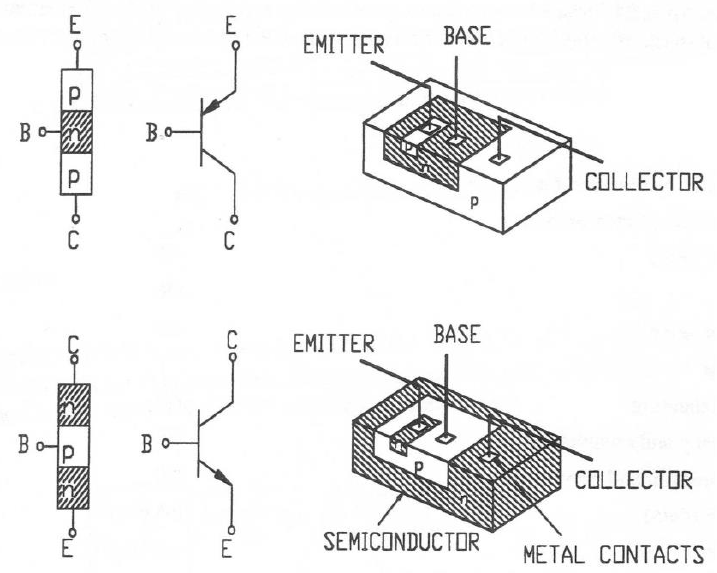
\includegraphics[width=0.5\linewidth]{structures_of_bjt.png}
		\captionof{figure}{Different Structures of BJT [1]}\label{f1}
	\end{figure}
	
	\subsection{BJT Operating Regions}
	As the BJT is a three-terminal device, there are basically three possible ways to connect it within an electronic circuit with one terminal being common to both the input and output.
	Figure \ref{f2} shows an example of an I-V curve of an NPN BJT transistor.\\
	As observed in Figure \ref{f2}, the effect of $V_{CE}$ upon the collector current ($I_C$), when $V_{CE}$ is greater than about 0.3 volts, is that $I_C$ is largely unaffected by changes in $V_{CE}$ and instead, it is almost entirely controlled by the base current [1].
	
	\begin{figure}[!ht]
		\centering
		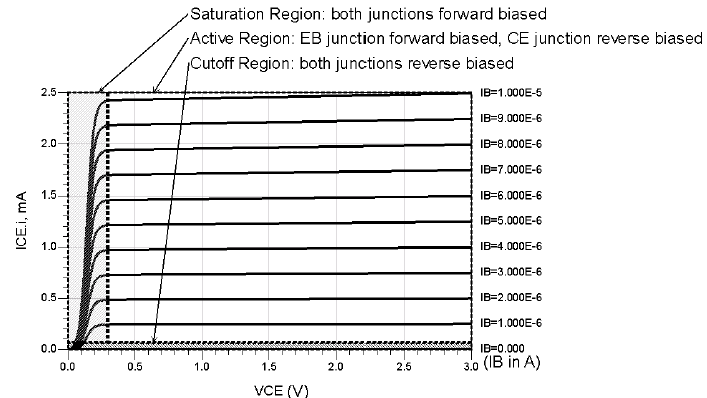
\includegraphics[width=0.7\linewidth]{I-V_characterization_curve.png}
		\captionof{figure}{I-V Curves of a BJT Sweeping $V_{CE}$ for different $I_B$ [1]}\label{f2}
	\end{figure}

	\noindent Figure \ref{f3} below shows the opposite type of curve, with a plot of collector current as the base-emitter voltage is swept [1].
	The collector-emitter voltage is held constant as this doesn’t affect the family of curves significantly.
	As the collector-emitter voltage changes to another constant, i.e. 5 volts, the base current ($I_B$) is barely affected by the change of collector-emitter voltage ($V_{CE}$).
	However, the base-emitter voltage ($V_{BE}$) needs to be around 0.7 volts in order to forward the PN junction between the base and the emitter which results in increasing the base current (IB) and therefore, an increase in the collector current ($I_C$).
	It is important to notice that a small change in the base current ($I_B$) will have a significant change in the collector current ($I_C$).
	
	\begin{figure}[!ht]
	\centering
	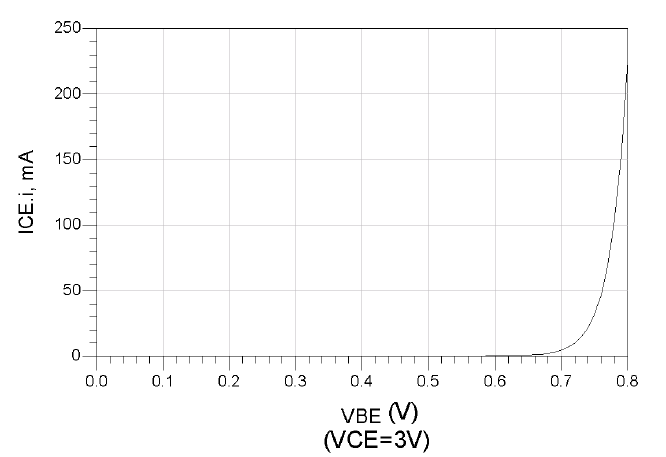
\includegraphics[width=0.6\linewidth]{I-V_diodelike_curve.png}
	\captionof{figure}{I-V Curves of a BJT Sweeping $V_{BE}$ for a fixed $V_{CE}$ [1]}\label{f3}
	\end{figure}

	\subsubsection{Saturation Region}
	In this region, both BE and BC junctions are forward biased [1].
	The collector-emitter voltage ($V_{CE}$) is small, a value of 0.2 volts or lower.
	However, a large collector and base currents ($I_C$ and $I_B$) can flow. 
	
	\subsubsection{Active Region}
	In this region, the BE junction is forward biased, but the BC junction is reversed biased [1].
	That transistor is used in this region for amplification.
	Since the two junctions are very close together, the emitter emits carriers which shoot across the central base region and are collected by the collector region.
	This lets the collector current be controlled almost completely by the base-emitter junction voltage and is nearly independent on the collector node voltage [1].
	They are governed by the following relation: $$\beta = \frac{I_C}{I_B}$$
	where,\\
	$\beta$ is the common-emitter current gain.\\
	$I_C$ is the collector current of the transistor.\\
	$I_B$ is the base current of the transistor.
	
	\subsubsection{Cutoff Region}
	In this region, both BE and BC junctions are reverse biased [1]. No current gain is available in this mode and there is a high resistance between the collector (C) and emitter (E) terminals.
	
	\vspace{2cm}	
	\noindent \textbf{Note} that \textbf{\textit{Multisim}} software was used to obtain all the presented data in this report.
	
	\pagebreak
	
	\section{BJT DC Characterization}
	\subsection{Diode-Like Behavior of BJT Junctions, and BJT Type}
	Figure \ref{f4} illustrates the use of a Digital Volt Meter (DVM) on the \textit{"diode"} setting to the measure the forward and reverse voltages of the B-E, B-C, and C-E junctions of both 2N3904 and 2N3906 transistors. 
	
	\begin{figure}[!ht]
		\centering
		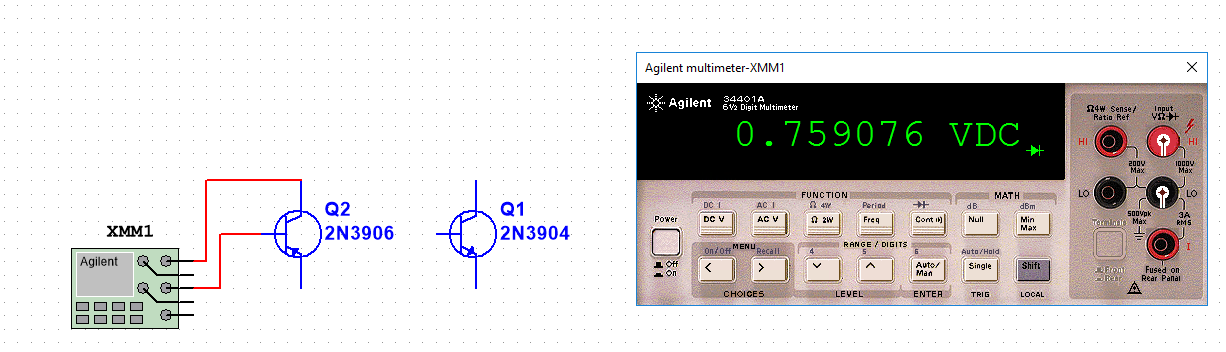
\includegraphics[width=\linewidth]{d1-part1.png}
		\captionof{figure}{The Use of DVM to Measure Junction Voltages}\label{f4}
	\end{figure}

	\noindent The forward and reverse biases volatages are measured for both 2N3904 and 2N3906 transistors.
	Note that all collected data are measured in volts and can be seen in Tables \ref{t1} and \ref{t2} below.
	
	\begin{table}[!ht]
		\centering
		\captionof{table}{2N3904 Transistor's Forward and Reverse Biases Voltages}\label{t1}
		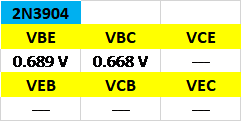
\includegraphics[width=0.4\linewidth]{d1-part1.1.png}
	\end{table}
	
	\begin{table}[!ht]
		\centering
		\captionof{table}{2N3906 Transistor's Forward and Reverse Biases Voltages}\label{t2}
		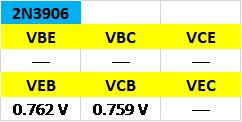
\includegraphics[width=0.4\linewidth]{d1-part1.2.png}
	\end{table}

	\noindent As observed from Table \ref{t1}, the transistor is seen to have a base-emitter voltage, $V_{BE}$, of approximately 0.7 volts which means that the base-emitter junction is forward biased and acts as a diode when the transistor is in active mode.
	The transistor is also seen to have a base-collector voltage, $V_{BC}$, that is less than $V_{BE}$ which means the the base-collector junction is reverse biased and acts like an open circuit blocking any current flow (only a very small leakage current).
	Due to that, the direction of the current is from the base to the emitter.
	Therefore, the 2N3904 transistor model is an NPN transistor.
	
	\pagebreak
		
	\noindent As observed from Table 2, the transistor is seen to have an emitter-base voltage, $V_{EB}$, of approximately 0.7 volts which means that the emitter-base junction is forward biased and acts as a diode when the transistor is in active mode.
	The transistor is also seen to have a collector-base voltage, $V_{CB}$, that is less than $V_{EB}$ volts which means the the collector-base junction is reverse biased and acts like an open circuit blocking any current flow (only a very small leakage current).
	Due to that, the direction of the current is from the emitter to the base.
	Therefore, the 2N3906 transistor model is an PNP transistor.
		
	\subsection{BJT $I_C$ vs. $V_{CE}$ Characteristic Curves -Point-by-Point- Plotting}
	\subsubsection{Prelab Calculations}
	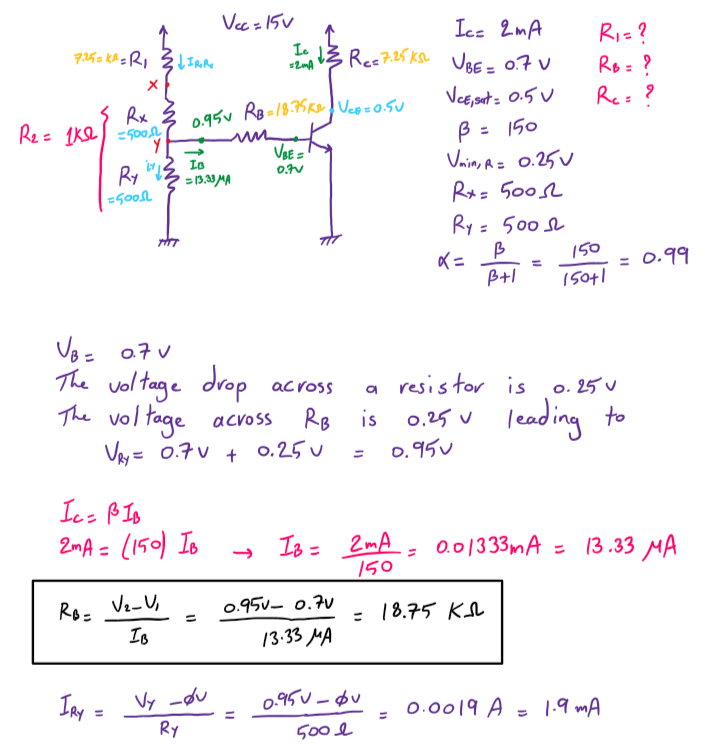
\includegraphics[width=\linewidth]{prelab1.png}
	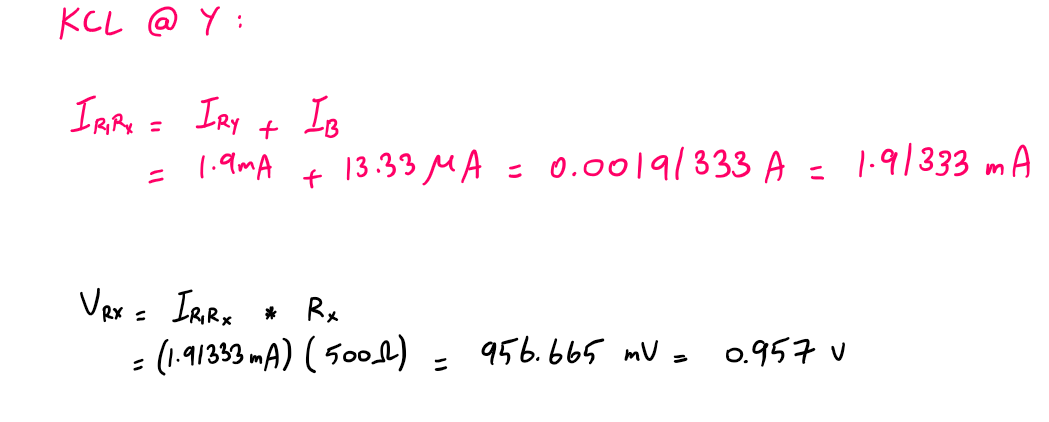
\includegraphics[width=\linewidth]{prelab2.png}
	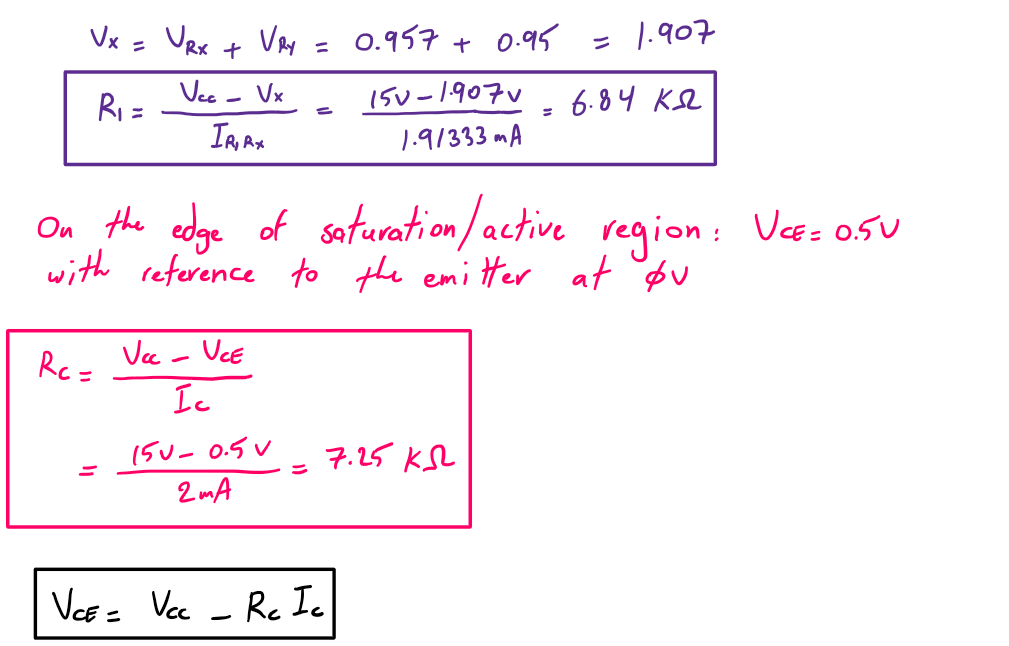
\includegraphics[width=\linewidth]{prelab3.png}
	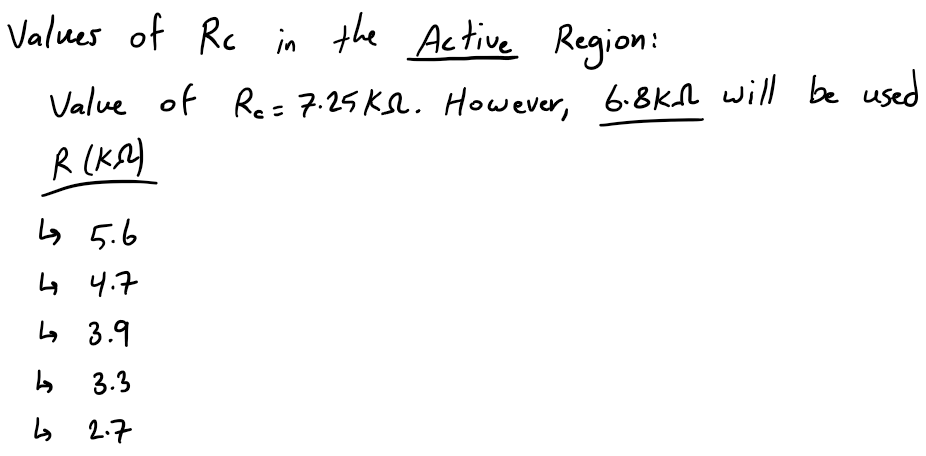
\includegraphics[width=\linewidth]{prelab4.png}
	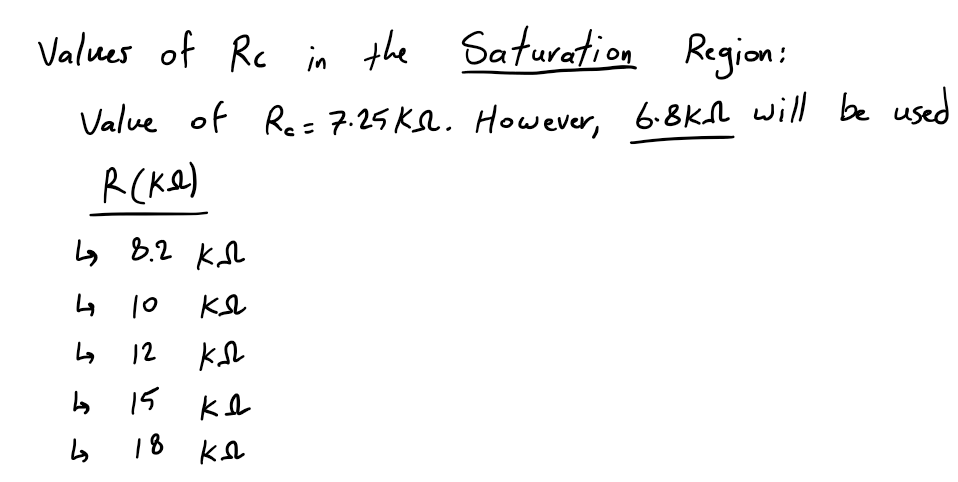
\includegraphics[width=\linewidth]{prelab5.png}
	
	\pagebreak
	
	\subsubsection{Experiment}
	Figure \ref{f5} below illustrates the test circuit used in this part of the experiment.
	
	\begin{figure}[!ht]
		\centering
		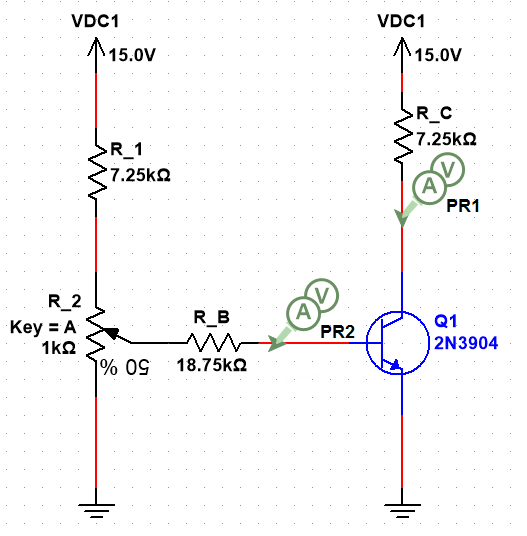
\includegraphics[width=0.6\linewidth]{d1-part2-circuit.png}
		\captionof{figure}{Test Circuit}\label{f5}
	\end{figure}
	
	\noindent Figure \ref{f6} below illustrates the DC operating sweep settings of the test circuit used in this part of the experiment.

	\begin{figure}[!ht]
		\centering
		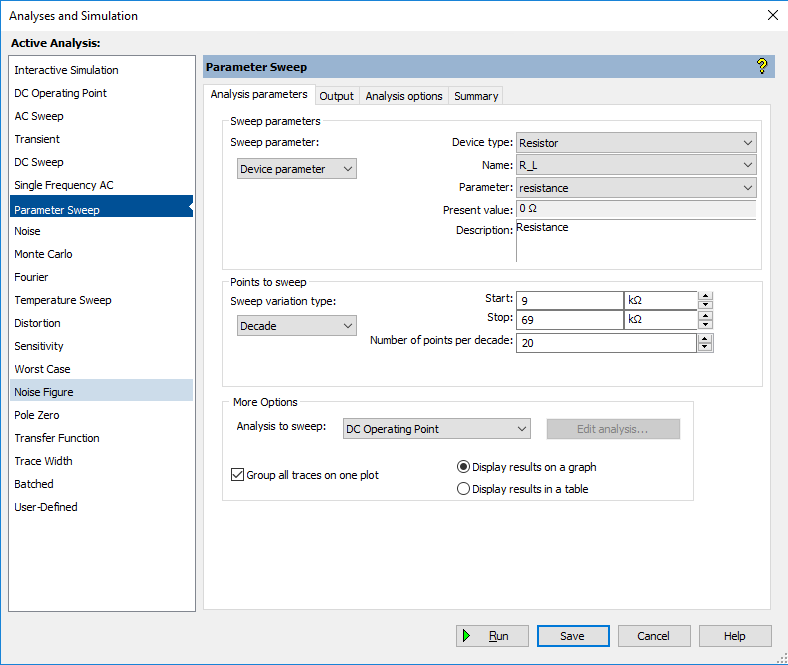
\includegraphics[width=0.55\linewidth]{d1-part2-DcOperatingSweep.png}
		\captionof{figure}{DC Operating Sweep Simulation Settings}\label{f6}
	\end{figure}	

	\noindent Table \ref{t3} below shows the measured collector current, $I_C$,, the base-emitter voltage, $V_{BE}$, and the collector-emitter voltage, $V_{CE}$, for different collector resistance values, $R_C$.
	Also, the table shows the calculations of the current ration $\beta$ for the transistor at each chosen $R_C$.

	\begin{table}[!ht]
		\centering
		\captionof{table}{Measured $I_C$, $V_{BE}$, and $V_{CE}$ for Different $R_C$ Values}\label{t3}
		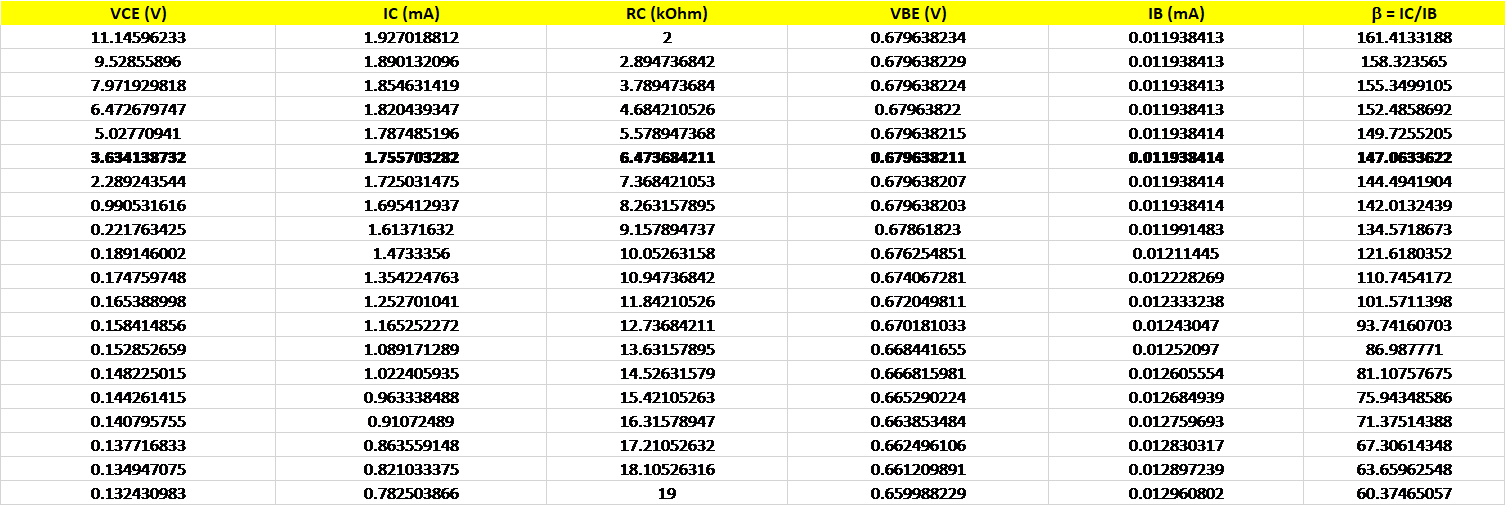
\includegraphics[width=\textwidth]{part2-data-measured}	
	\end{table}	

	\noindent Figure \ref{f7} below shows the plot of $I_C$-$V_{CE}$ line for the base current that was held constant.
	\begin{figure}[!ht]
		\centering
		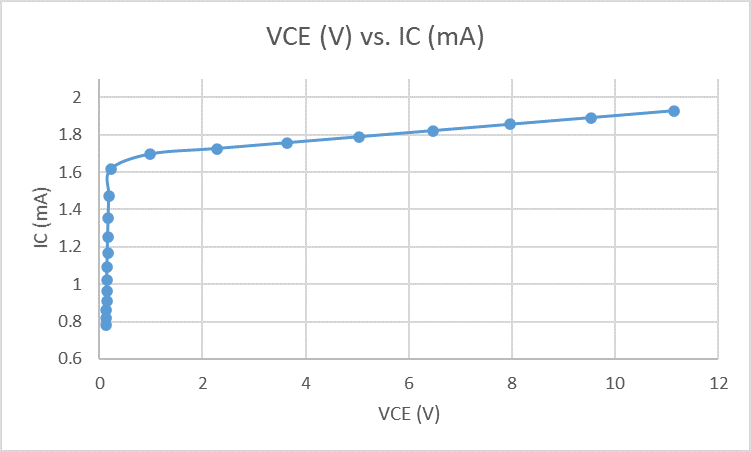
\includegraphics[width=0.8\linewidth]{vce_vs_ic.png}
		\captionof{figure}{Collector-Emitter Voltage vs. Collector Current}\label{f7}
	\end{figure}

	\pagebreak

	\noindent Figure \ref{f8} below shows the plot of $V_{BE}$ vs. $V_{CE}$.
	\begin{figure}[!ht]
		\centering
		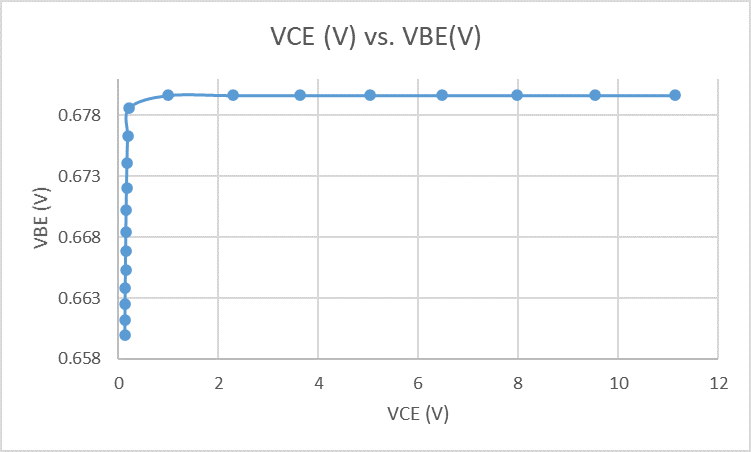
\includegraphics[width=0.8\linewidth]{vce_vs_vbe.png}
		\captionof{figure}{Collector-Emitter Voltage vs. Base-Emitter Voltage}\label{f8}
	\end{figure}
	
	\noindent As observed from Figure \ref{f8}, the base-emitter voltage, $V_{BE}$, remains approximately constant as, $V_{CE}$, increases when the BJT is operating in the active region.
	While the BJT remains in the active mode, the base-emitter junction acts as a diode and thus will always have a voltage of approximately 0.7 volts across it.
	However, when the BJT operates in the saturation region, the base-emitter voltage, $V_{BE}$, slowly decreases.\\\\
	As seen in Table \ref{t3} before, increasing the collector resistance values, $R_C$, to a value that is higher than 7.25 k$\Omega$, the collector current, $I_C$, decreases while the base current, $I_B$, remains constant which results in a smaller current ratio.\\\\
	As seen in Table 3 before, the current ration ${I_C}/{I_B}$ was calculated for all the value of $R_C$, and the approximate $\beta$ value when the transistor is operating in the active region is \textbf{147.06}.
	
	\pagebreak
	
	\noindent In order to find the Early voltage ($V_A$), values are taken from Table \ref{t3} and plotted when the BJT is operating in the active region.
	The Early voltage is the x-intercept of the trendline in Figure \ref{f9}.
	
	\begin{figure}[!ht]
		\centering
		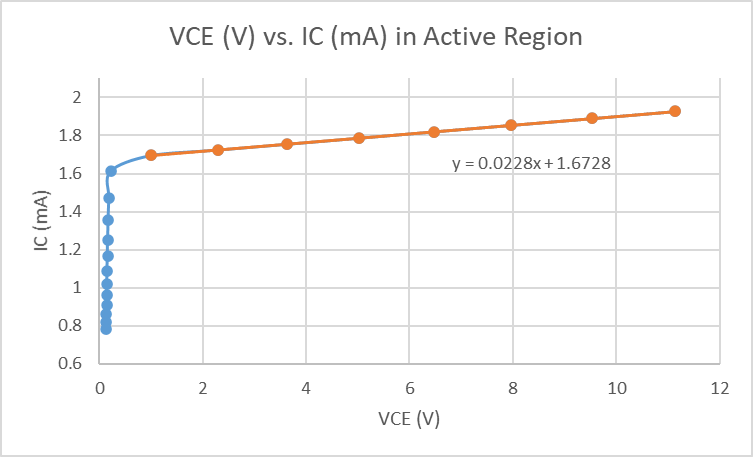
\includegraphics[width=0.8\linewidth]{vce_vs_ic_slope.png}
		\captionof{figure}{Collector-Emitter Voltage vs. Collector Current in the Active Region}\label{f9}
	\end{figure}
	
	\noindent The slope of Figure \ref{f9} is the value of the output admittance, 1/$r_o$, and the x-intercept of the slope equation is the value of the Early voltage ($V_A$).\\\\
	Using the slope equation of Figure \ref{f9}:
	$$y = 0.0228x + 1.6728$$
	By setting the y-value to zero, the x-intercept is calculated as follows:
	$$0 = 0.0228x + 1.6728$$
	$$x = \frac{-1.6728}{0.0228} = -73.37$$\\\\
	The Early voltage is the absolute value of \textbf{-73.37} volts.
	\pagebreak
	
	\subsection{The Current Mirror}
	\subsubsection{Prelab Calculations}
	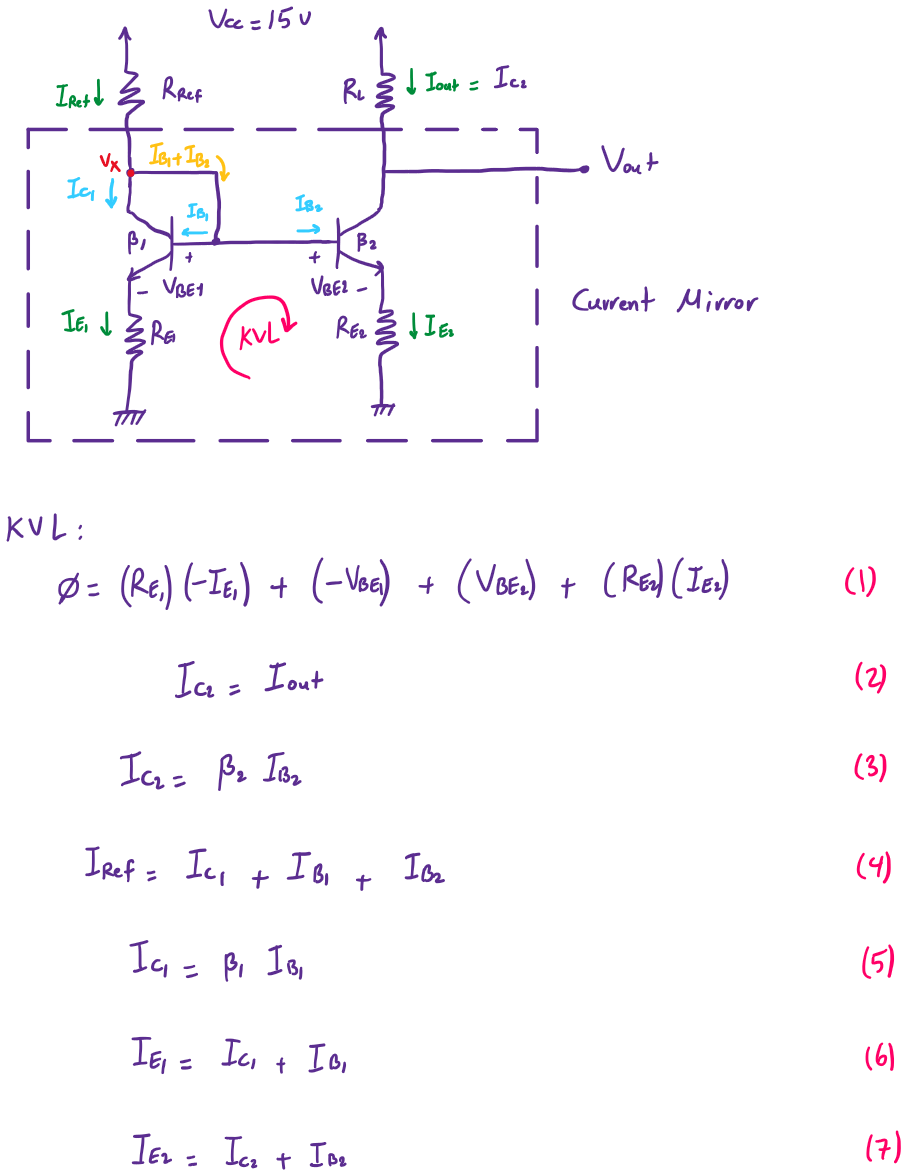
\includegraphics[width=\linewidth]{prelab6.png}
	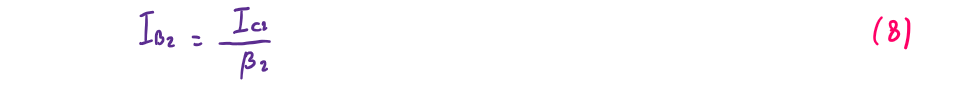
\includegraphics[width=\linewidth]{prelab7.png}
	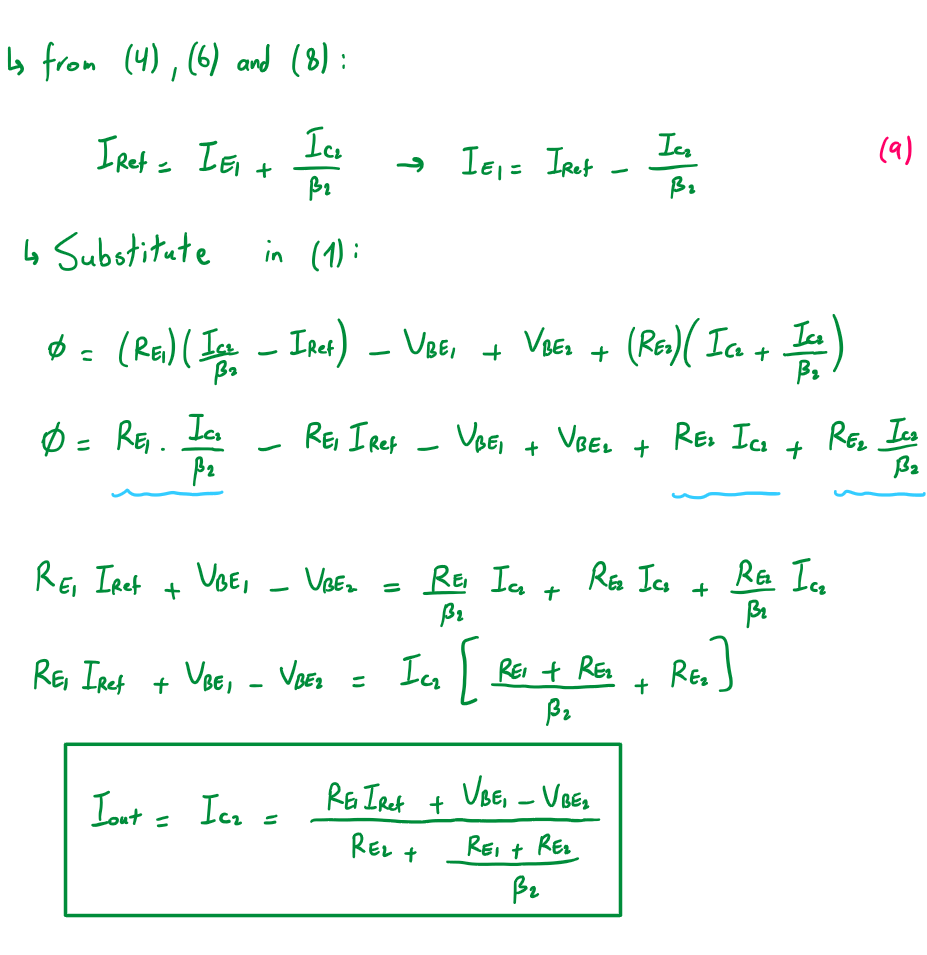
\includegraphics[width=\linewidth]{prelab8.png}
	
\includegraphics[width=\linewidth]{prelab9.png}
	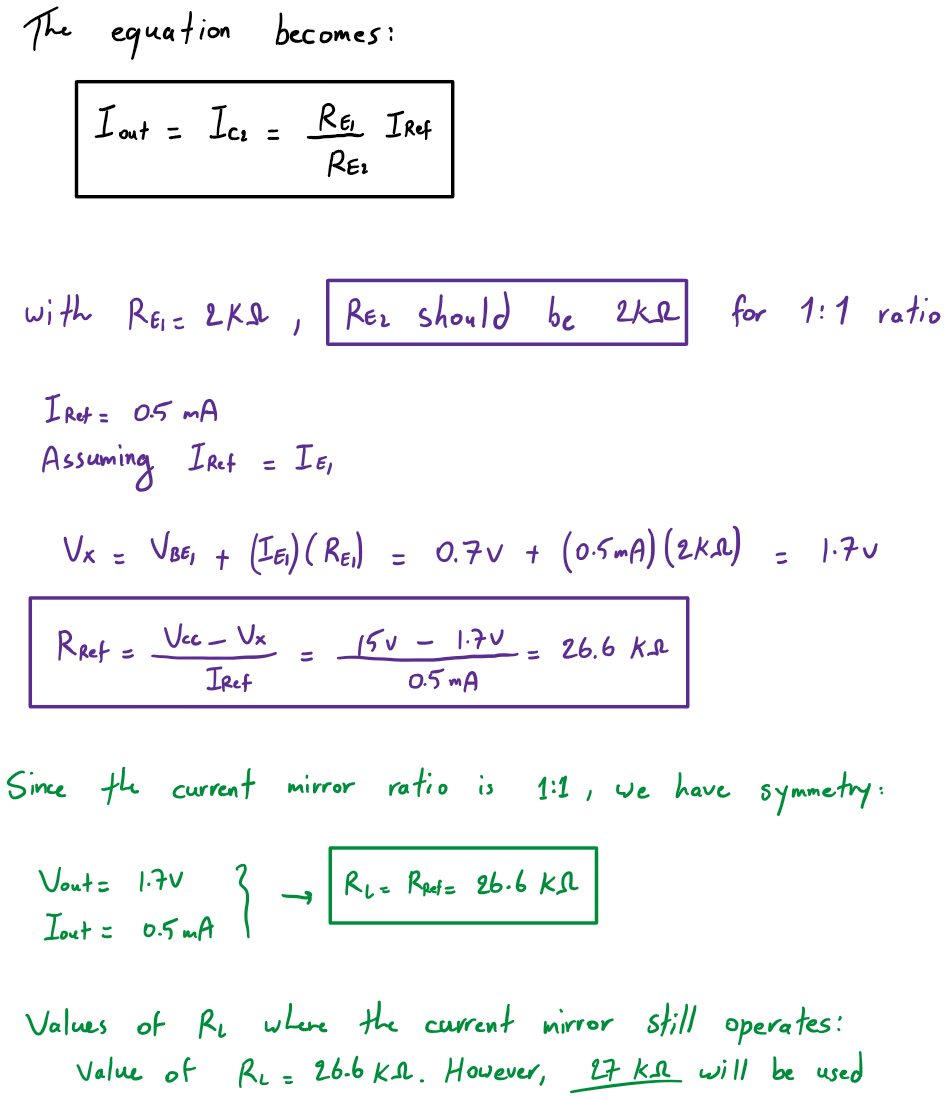
\includegraphics[width=\linewidth]{prelab10.png}
	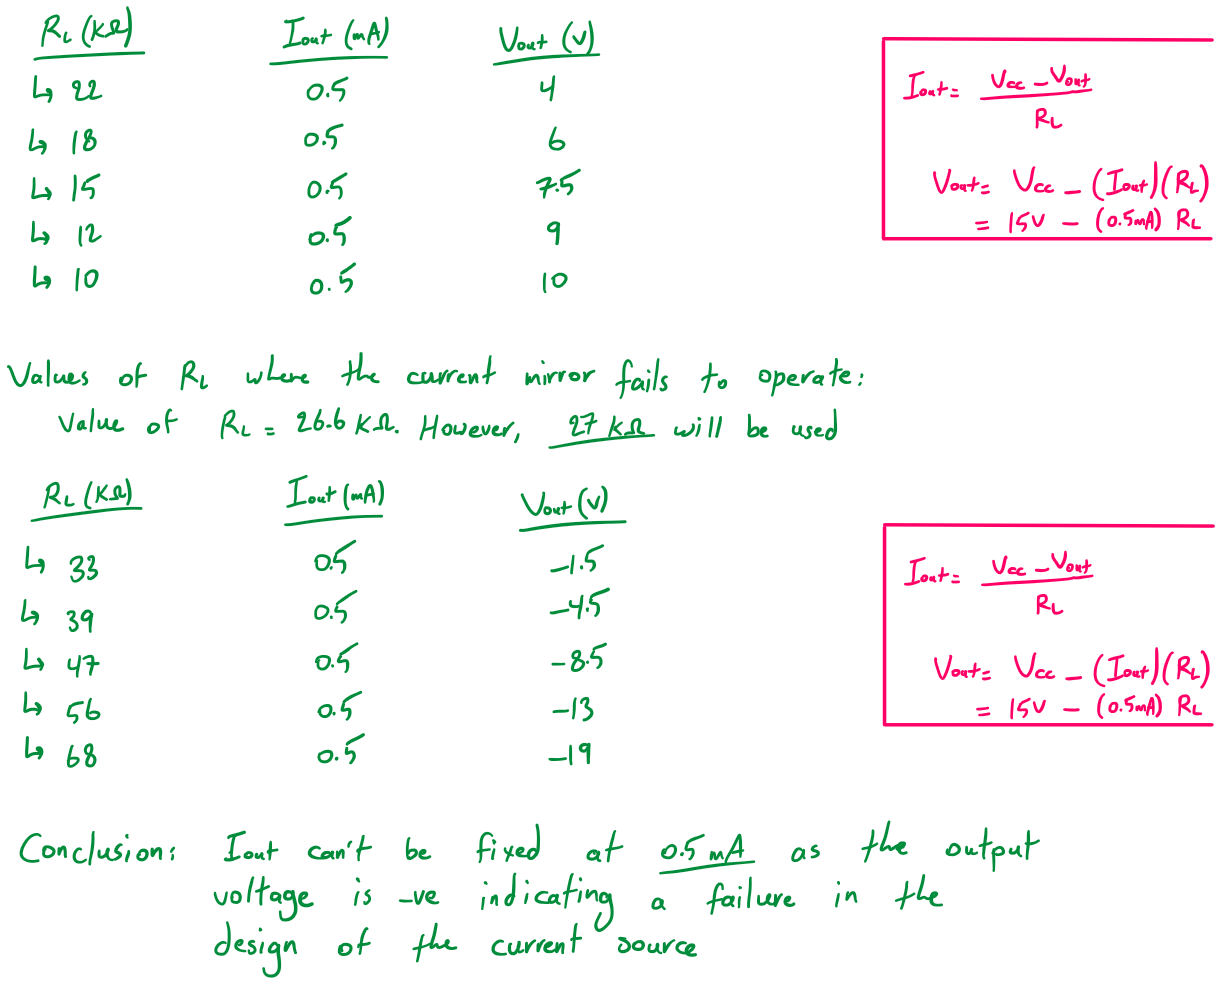
\includegraphics[width=\linewidth]{prelab11.png}
	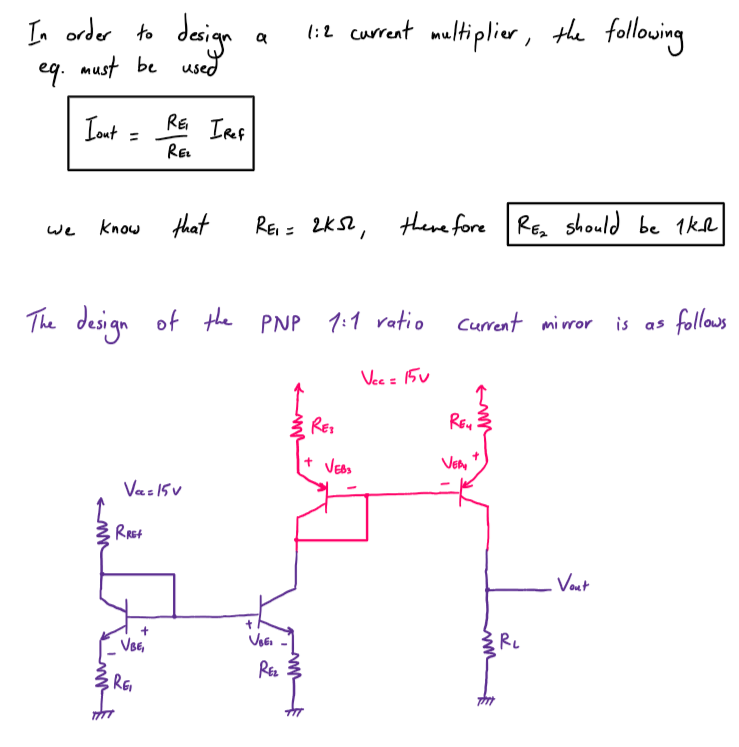
\includegraphics[width=\linewidth]{prelab12.png}
	
	\pagebreak
	
	\subsubsection{Experiment: 1:1 NPN Current Multipllier}
	Figure \ref{f10} below illustrates the current mirror circuit used in this part of the experiment.
	\begin{figure}[!ht]
		\centering
		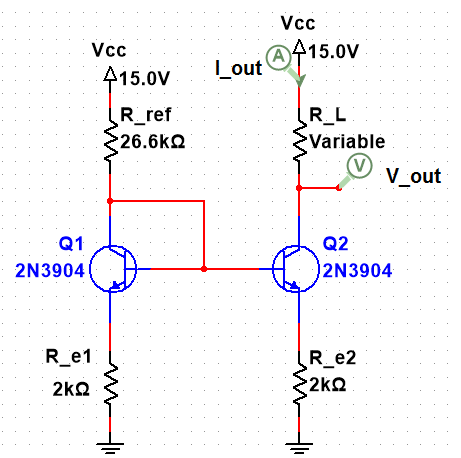
\includegraphics[width=0.57\linewidth]{d1-part3-circuit-npn-1_1.png}
		\captionof{figure}{The 1:1 Ratio NPN Current Mirror Circuit}\label{f10}
	\end{figure}
	
	\noindent Figure \ref{f11} below illustrates the DC operating sweep settings of the 1:1 ratio current mirrior circuit used in this part of the experiment.
	\begin{figure}[!ht]
		\centering
		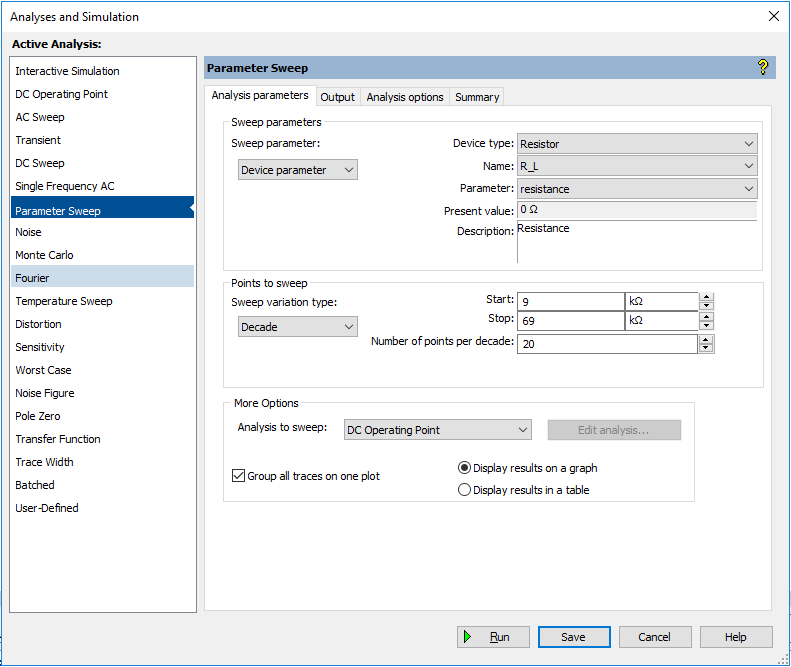
\includegraphics[width=0.6\linewidth]{d1-part3-DcOperatingSweep.png}
		\captionof{figure}{The 1:1 Ratio NPN DC Operating Sweep Simulation Settings}\label{f11}
	\end{figure}
		
	\pagebreak
	
	\noindent For the 1:1 ratio NPN current mirror, the reference resistance, $R_{REF}$, is set to be 26.6 k$\Omega$ and the reference voltage was measured and found to be 13.4 volts.
	Therefore, the reference current, $I_{REF}$, can be calculated as follows: $$I_{REF} = \frac{V_{REF}}{R_{REF}} = \frac{13.4 V}{26.6 k\Omega} = 0.50$$
	Therefore, the reference current, $I_{REF}$, for the 1:1 ratio multiplier is \textbf{0.50 mA}.\\\\	
	Table \ref{t4} below shows the output current of the 1:1 current mirror circuit with different values of the load resistor when the transistor is operating in both active and saturation regions.
	\begin{table}[!ht]
		\centering
		\captionof{table}{Measured $I_{OUT}$ and $V_{OUT}$ for Different $R_L$ Values for 1:1 Ratio NPN}\label{t4}
		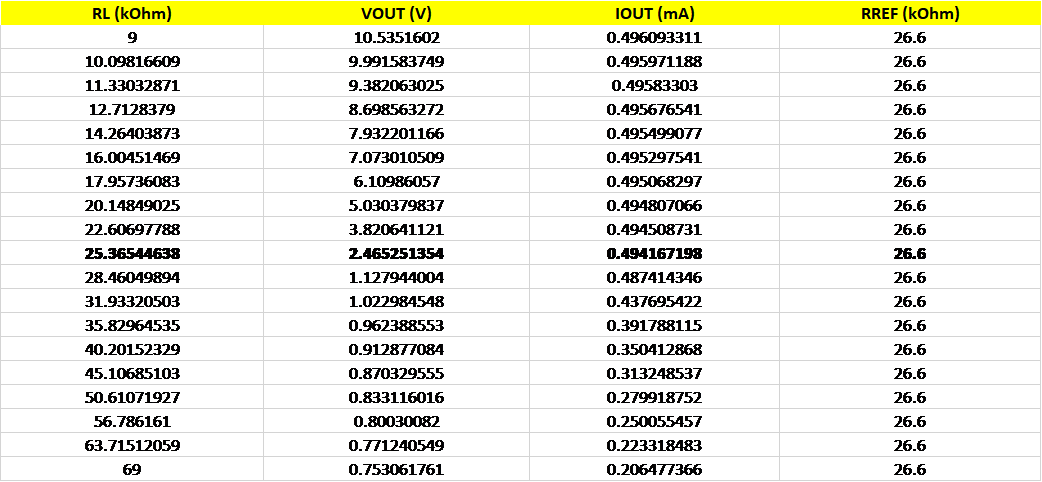
\includegraphics[width=\linewidth]{part3-data-measured-npn-1_1.png}	
	\end{table}
	
	\pagebreak
	
	\noindent Figure \ref{f12} below shows how the output current, $I_{OUT}$, remains constant and equals to the reference current, $I_{REF}$, for any load resistance values as long as the transistor is operation in the active region.
	The maximum load resistance value, $R_{L_{MAX}}$, is \textbf{26.6 k$\Omega$}.
	Any chosen load resistance values, $R_L$, that are higher than $R_{L_{MAX}}$ will make the transistor operate in the saturation region.
	In this case, the current mirror fails and the output current, $I_{OUT}$, will decrease as observed in Table \ref{t4}.
	\begin{figure}[!ht]
		\centering
		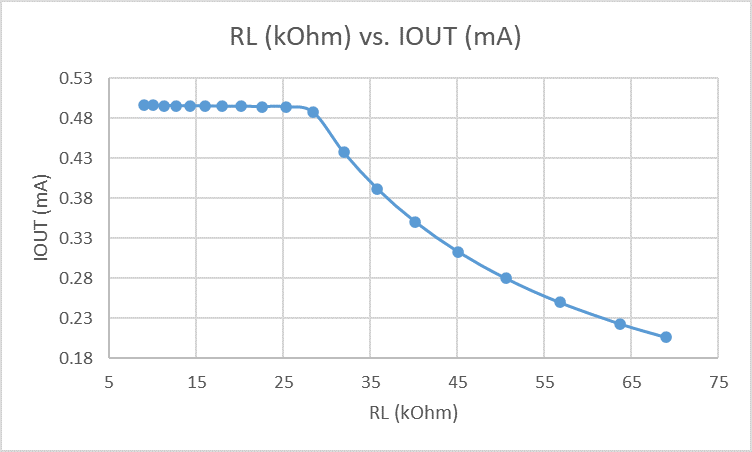
\includegraphics[width=0.8\linewidth]{iout_vs_rl_1_1.png}
		\captionof{figure}{Load Resistor vs. Output Current for 1:1 Ratio NPN}\label{f12}
	\end{figure}	

	\noindent Figure \ref{f13} below shows a plot of the output voltage vs. output current.
	\begin{figure}[!ht]
		\centering
		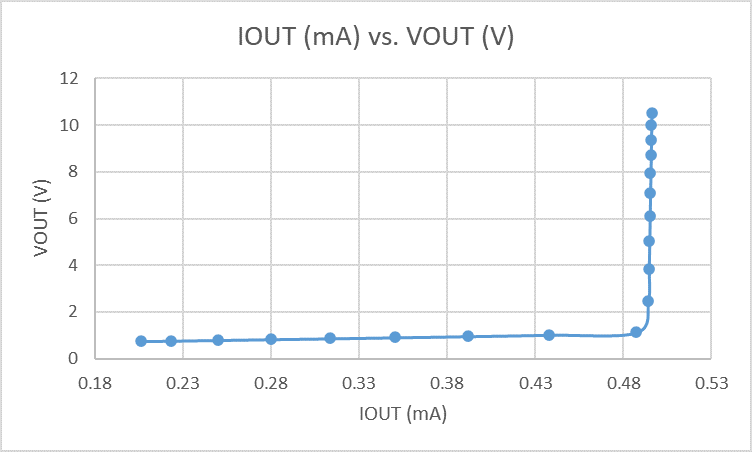
\includegraphics[width=0.8\linewidth]{iout_vs_vout.png}
		\captionof{figure}{Output Current vs. Output Voltage for 1:1 Ratio NPN}\label{f13}
	\end{figure}
	
	\noindent In order to determine the output impedance, values are taken from Table \ref{t4} and plotted when the BJT is operating in the active region.
	The output impedance is 1 divided by the slope of the trendline in Figure \ref{f14}.
	
	\begin{figure}[!ht]
		\centering
		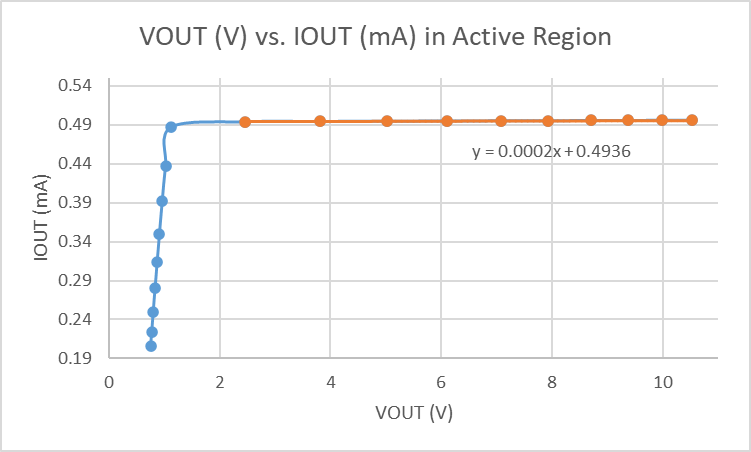
\includegraphics[width=0.8\linewidth]{vout_vs_iout_slope.png}
		\captionof{figure}{Output Voltage vs. Output Current in the Active Region for 1:1 Ratio NPN}\label{f14}
	\end{figure}
	
	\pagebreak
	
	\noindent Using Figure \ref{f14} above, when the transistor is in active mode, the $I_{OUT}$ vs. $V_{OUT}$ relationship appears to have a slope of approximately \textbf{0.000238} (the slope of the data when the BJT is only in active mode). The output impedance can be calculated as follows: $$Output \hspace{1mm} Impedance = \frac{1}{m} = \frac{1}{0.000238 * 10^{-3}} = 4,201,680.67$$
	The output impedance is \textbf{4,201,680.67 mhos}.
	
	\pagebreak
	
	\subsubsection{Experiment: 1:2 NPN Current Multipllier}
	Figure \ref{f15} below illustrates the current mirror circuit used in this part of the experiment.
	\begin{figure}[!ht]
		\centering
		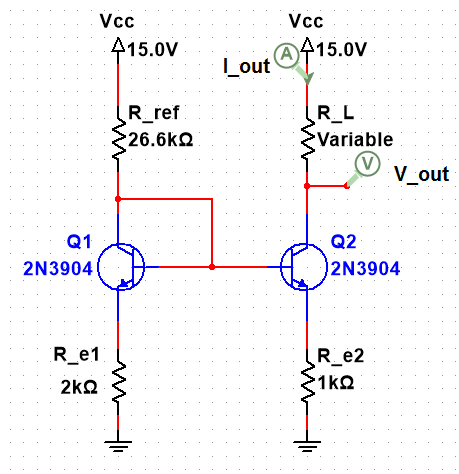
\includegraphics[width=0.55\linewidth]{d1-part3-circuit-npn-1_2.png}
		\captionof{figure}{The 1:2 Ratio NPN Current Mirror Circuit}\label{f15}
	\end{figure}
	
	\noindent Figure 16 below illustrates the DC operating sweep settings of the 1:2 ratio current mirrior circuit used in this part of the experiment.
	\begin{figure}[!ht]
		\centering
		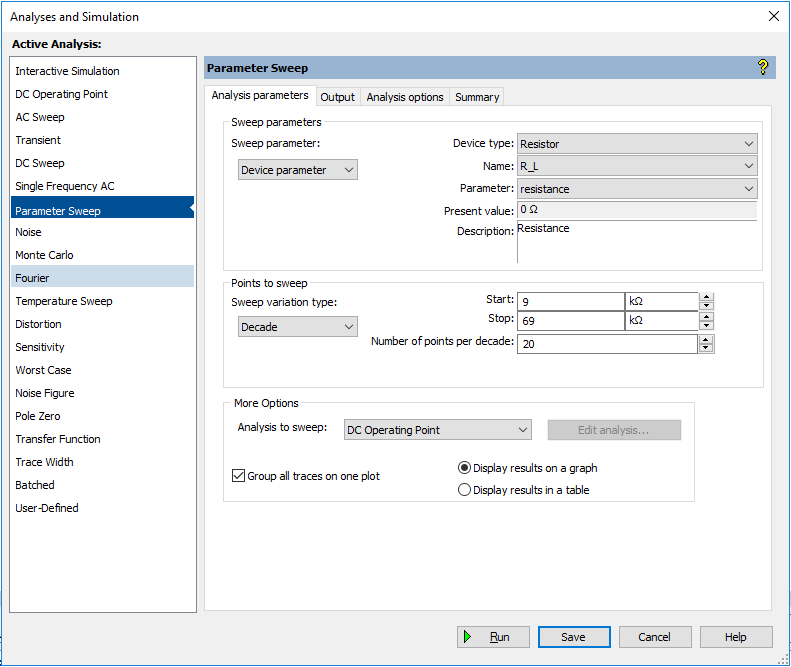
\includegraphics[width=0.62\linewidth]{d1-part3.1-DcOperatingSweep.png}
		\captionof{figure}{The 1:2 NPN DC Operating Sweep Simulation Settings}\label{f16}
	\end{figure}
	
	\pagebreak
	
	\noindent For the 1:2 ratio NPN current mirror, the reference resistance, $R_{REF}$, is set to be 26.6 k$\Omega$ and the reference voltage was measured and found to be 13.4 volts.
	Therefore, the reference current, $I_{REF}$, can be calculated as follows: $$I_{REF} = \frac{V_{REF}}{R_{REF}} = \frac{13.4 V}{26.6 k\Omega} = 0.50$$
	Therefore, the reference current, $I_{REF}$, for the 1:2 ratio multiplier is \textbf{0.50 mA}.\\\\
	Table \ref{t5} below shows the output current of the 1:2 current mirror circuit with different values of the load resistor when the transistor is operating in both active and saturation regions.
	\begin{table}[!ht]
		\centering
		\captionof{table}{Measured $I_{OUT}$ and $V_{OUT}$ for Different $R_L$ Values for 1:2 Ratio NPN}\label{t5}
		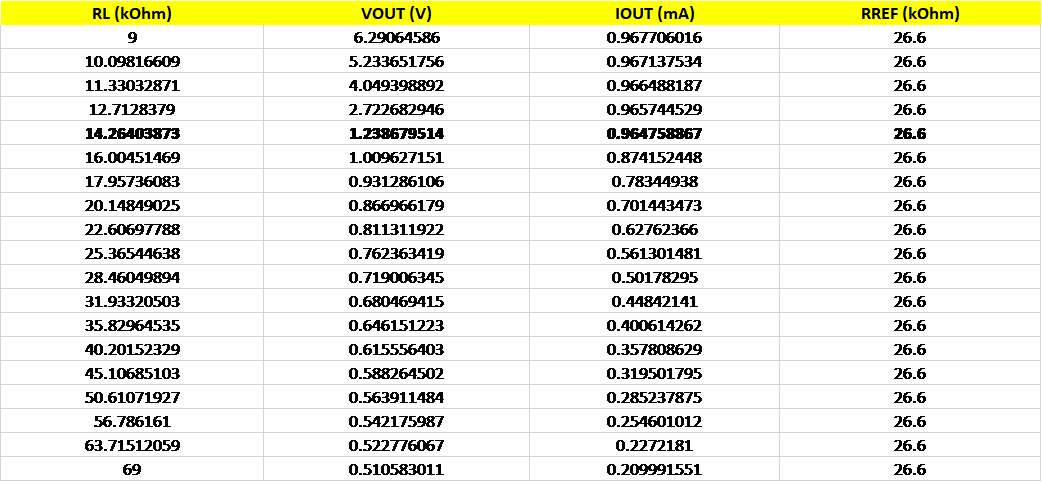
\includegraphics[width=\linewidth]{part3-data-measured-npn-1_2.png}
	\end{table}
	
	\pagebreak
	
	\noindent Figure \ref{f17} below shows how the output current, $I_{OUT}$, is equal to approximately 1 mA which is \textbf{\textit{double}} the reference current, $I_{REF}$, for any load resistance values as long as the transistor is operation in the active region.
	The maximum load resistance value, $R_{L_{MAX}}$, is appromximately \textbf{15 k$\Omega$}.
	Any chosen load resistance values, $R_L$, that are higher than $R_{L_{MAX}}$ will make the transistor operate in the saturation region.
	In this case, the current mirror fails and the output current, $I_{OUT}$, will decrease as observed in Table \ref{t5}.
	
	\begin{figure}[!ht]
		\centering
		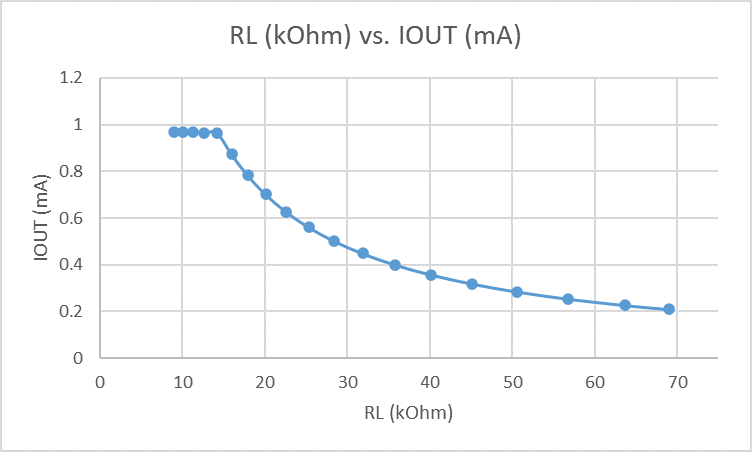
\includegraphics[width=0.8\linewidth]{iout_vs_rl_1_2.png}
		\captionof{figure}{Load Resistor vs. Output Current for 1:2 Ratio NPN}\label{f17}
	\end{figure}
	
	\pagebreak
	
	\subsubsection{Experiment: 1:1 NPN-PNP Current Multipllier}
	Figure \ref{f18} below illustrates the current mirror circuit used in this part of the experiment.
	\begin{figure}[!ht]
		\centering
		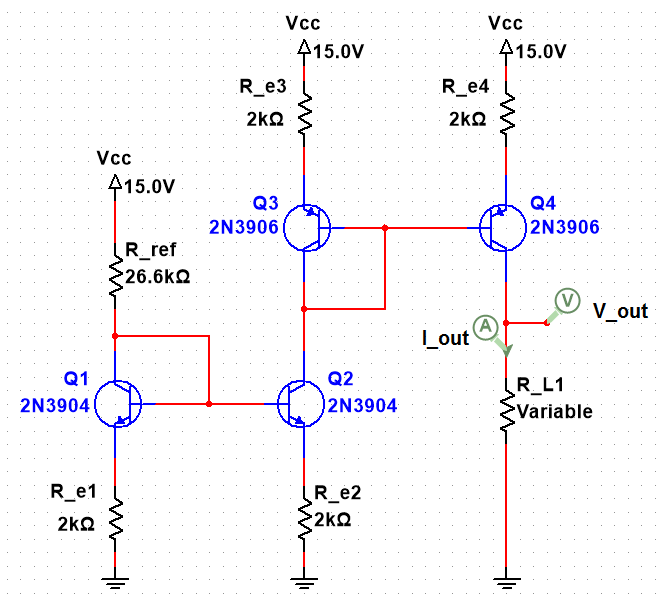
\includegraphics[width=0.6\linewidth]{d1-part3-circuit-npn_pnp-1_1.png}
		\captionof{figure}{The 1:1 Ratio NPN-PNP Current Mirror Circuit}\label{f18}
	\end{figure}
	
	\noindent Figure \ref{f19} below illustrates the DC operating sweep settings of the 1:2 ratio current mirrior circuit used in this part of the experiment.
	\begin{figure}[!ht]
		\centering
		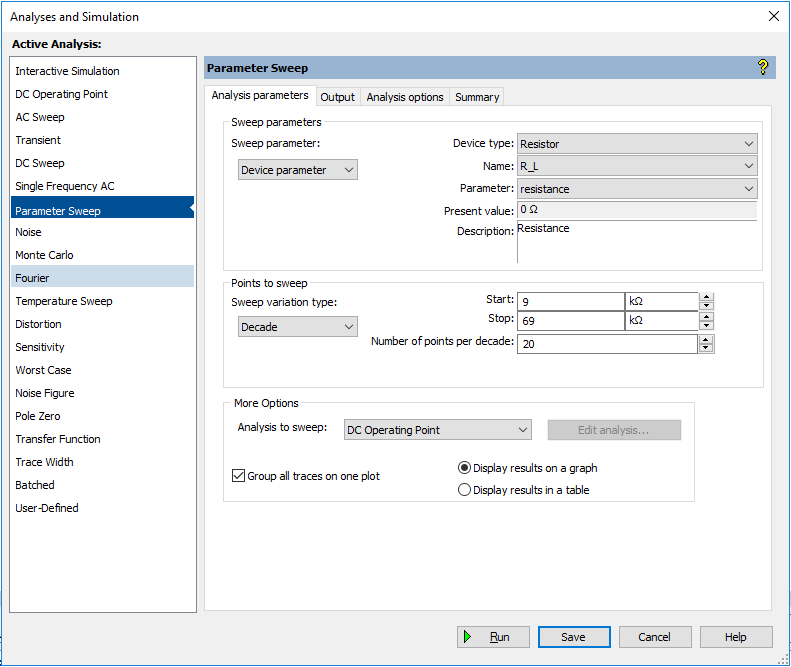
\includegraphics[width=0.64\linewidth]{d1-part3-DcOperatingSweep.png}
		\captionof{figure}{The 1:1 NPN-PNP DC Operating Sweep Simulation Settings}\label{f19}
	\end{figure}
	
	\pagebreak
	
	\noindent For the 1:1 ratio NPN-PNP current mirror, the reference resistance, $R_{REF}$, is set to be 26.6 k$\Omega$ and the reference voltage was measured and found to be 13.4 volts.
	Therefore, the reference current, $I_{REF}$, can be calculated as follows: $$I_{REF} = \frac{V_{REF}}{R_{REF}} = \frac{13.4 V}{26.6 k\Omega} = 0.50$$
	Therefore, the reference current, $I_{REF}$, for the 1:1 ratio multiplier is \textbf{0.50 mA}.\\\\
	Table \ref{t6} below shows the output current of the 1:1 NPN-PNP current mirror circuit with different values of the load resistor when the transistor is operating in both active and saturation regions.
	\begin{table}[!ht]
		\centering
		\captionof{table}{Measured $I_{OUT}$ and $V_{OUT}$ for Different $R_L$ Values for 1:1 Ratio NPN-PNP}\label{t6}
		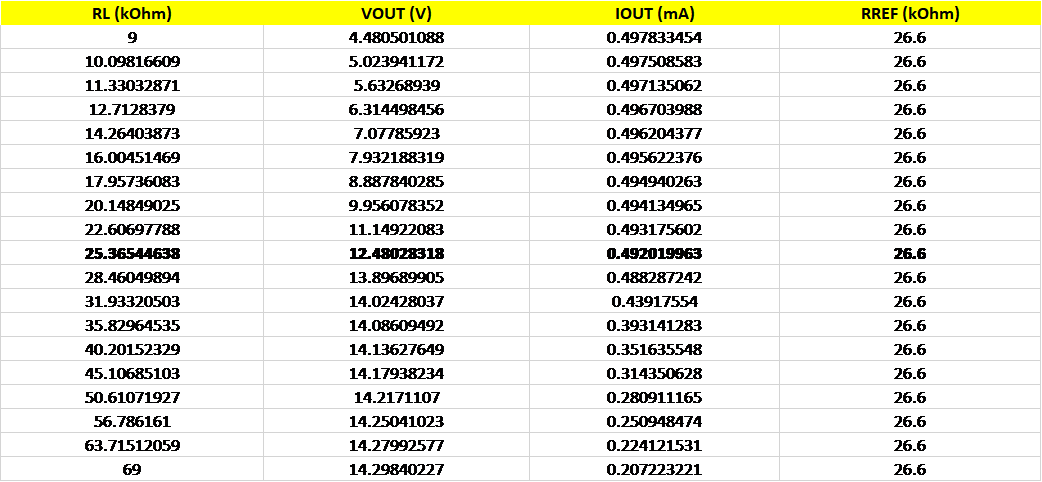
\includegraphics[width=\linewidth]{part3-data-measured-npn_pnp-1_1.png}
	\end{table}

	\pagebreak
	
	\noindent Figure \ref{f20} below shows how the output current, $I_{OUT}$, remains constant and equals to the reference current, $I_{REF}$, for any load resistance values as long as the transistor is operation in the active region.
	The maximum load resistance value, $R_{L_{MAX}}$, is \textbf{26.6 k$\Omega$}.
	Any chosen load resistance values, $R_L$, that are higher than $R_{L_{MAX}}$ will make the transistor operate in the saturation region.
	In this case, the current mirror fails and the output current, $I_{OUT}$, will decrease as observed in Table \ref{t6}.
	
	\begin{figure}[!ht]
		\centering
		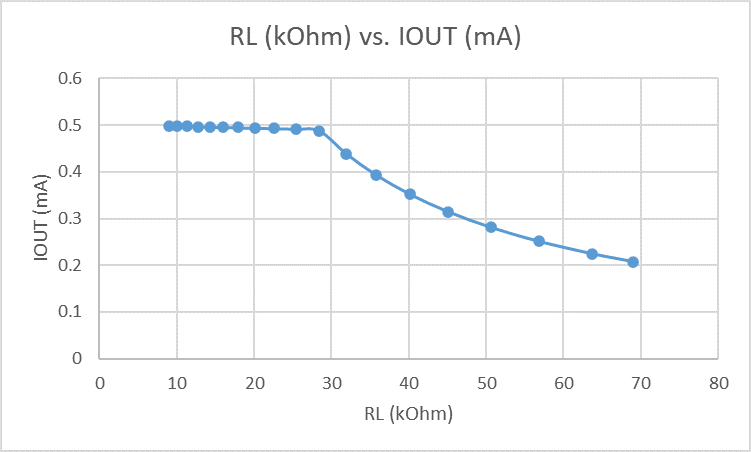
\includegraphics[width=0.8\linewidth]{iout_vs_rl_1_1_npnp.png}
		\captionof{figure}{Load Resistor vs. Output Current for 1:1 Ratio NPN-PNP}\label{f20}
	\end{figure}
	
	\pagebreak
	
	\section{BJT AC Characterization}
	\subsection{The transistor's h-Parameters and Bandwidth}
	The four h-parameters describe all of a transistor's small-signal ac characteristics for a given set of dc bias conditions, at one frequency [1].
	At low to medium frequencies, they are independent of frequency [1].\\\\
	The four parameters are:
	\begin{itemize}
		\item $h_{ie}$: the ac input impedance with the output short-circuited
		\item $h_{oe}$: the output admittance with the input open-circuited
		\item $h_{fe}$: the ac forward current gain with the output short-circuited
		\item $h_{re}$: the reverse, or feedback, voltage ratio with the input open-circuited		
	\end{itemize}
	The second subscript, \textbf{e}, indicates that these parameters are measured with respect to the emitter, the emitter being the terminal common to both the input circuit and the output circuit [1].\\\\
	The one other transistor parameter of major interest is its unity-gain bandwidth, $f_T$, the frequency at which its ac current gain is reduced to one [1].
	In this lab report, $f_T$ will be calculated as the product of the low-frequency current gain, $h_{fe}$, and the beta cut-off frequency, $f_{\beta}$.
	
	\subsubsection{DC-Biasing Circuit}
	Figure \ref{f21} below illustrates the circuit used in this part of the experiment.
	\begin{figure}[!ht]
		\centering
		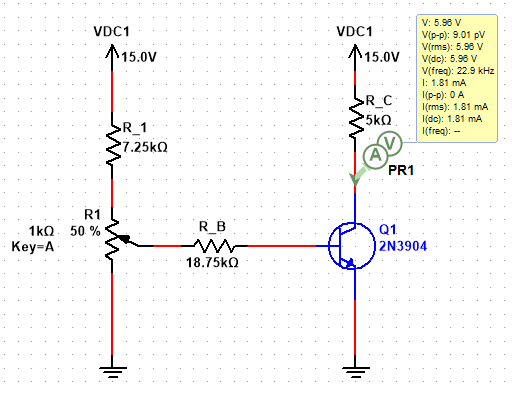
\includegraphics[width=0.8\linewidth]{part4-a1.png}
		\captionof{figure}{DC Bias Circuit for the AC Characterization Tests}\label{f21}
	\end{figure}
	
	\pagebreak
	
	\noindent Figure \ref{f22} below illustrates the interactive simulation settings of the DC Bias Circuit used in this part of the experiment.
	\begin{figure}[!ht]
		\centering
		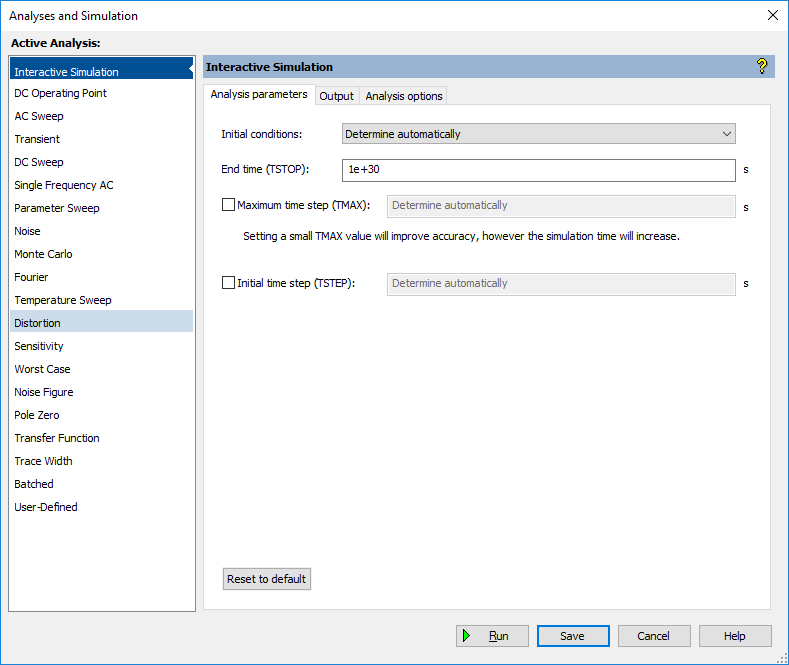
\includegraphics[width=0.55\linewidth]{part4-DcOperatingSweep.png}
		\captionof{figure}{The Interactive Simulation Settings of the DC Bias Circuit}\label{f22}
	\end{figure}
	
	\noindent As shown in Figure \ref{f21} above, the collector resistor, $R_C$, was set to \textbf{5 k$\Omega$} to maintain a collector-emitter voltage, $V_{CE}$, of approximately 6 volts.\\\\
	Then, the potentiometer percentage was adjusted to 48\% so that the collector current, $I_C$, is set to approximately 2 mA.\\\\
	As shown in Figure \ref{f23} below, the actual collector-emitter voltage ($V_{CE}$) was measured and found to be \textbf{4.70 volts}.
	\begin{figure}[!ht]
		\centering
		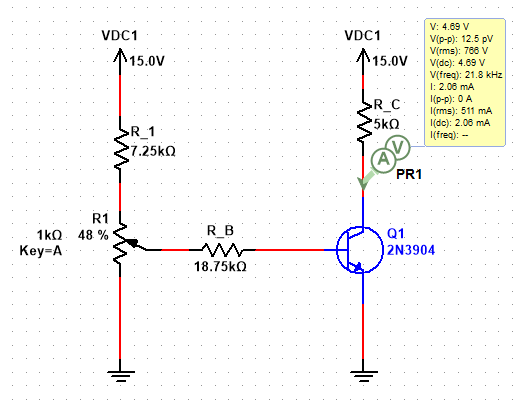
\includegraphics[width=0.6\linewidth]{part4-a2}
		\captionof{figure}{Measured $V_{CE}$ After Adjusting $I_C$ to 2 mA}\label{f23}
	\end{figure}

	\pagebreak
	
	\subsubsection{AC-Coupling of Input and Output Signals}
	Figure \ref{f24} below illustrates the circuit used in this part of the experiment.
	\begin{figure}[!ht]
		\centering
		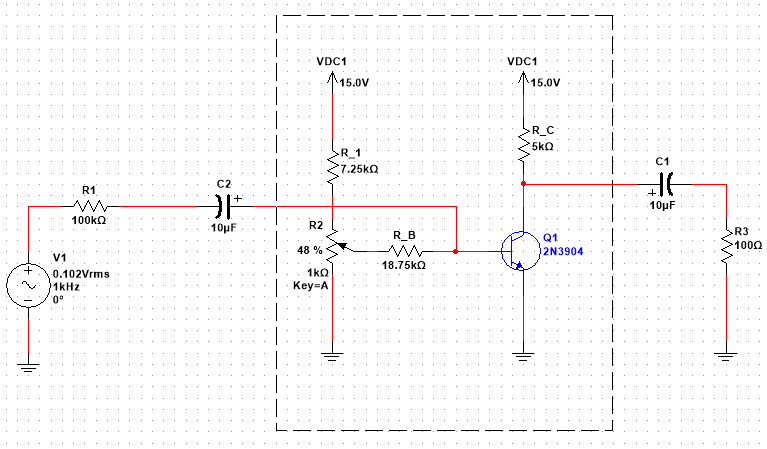
\includegraphics[width=0.8\linewidth]{part4-b-circuit.png}
		\captionof{figure}{Additional Circuitry Added to The DC Bias Circuit}\label{f24}
	\end{figure}
	
	\noindent Figure \ref{f24} above shows the AC test circuit for the biased BJT which has two capacitors, C1 and C2.
	These capacitors are used to block the DC signal from going to the test circuit.
	If the capacitors were not present, the resistors, $R_S$ and $R_L$, would experience DC voltage combined with the AC voltage signal.
	The DC voltage is only used to determining the biasing point of the cirucit and it is not desired when AC analysis is being done.
	
	\pagebreak
	
	\subsubsection{The AC Input Impedance, $h_{ie}$, and the AC Forward Current Gain, $h_{fe}$}
	Figure \ref{f25} below illustrates the interactive simulation settings of the test circuit, see Figure \ref{f24} above, used in this part of the experiment.
	\begin{figure}[!ht]
		\centering
		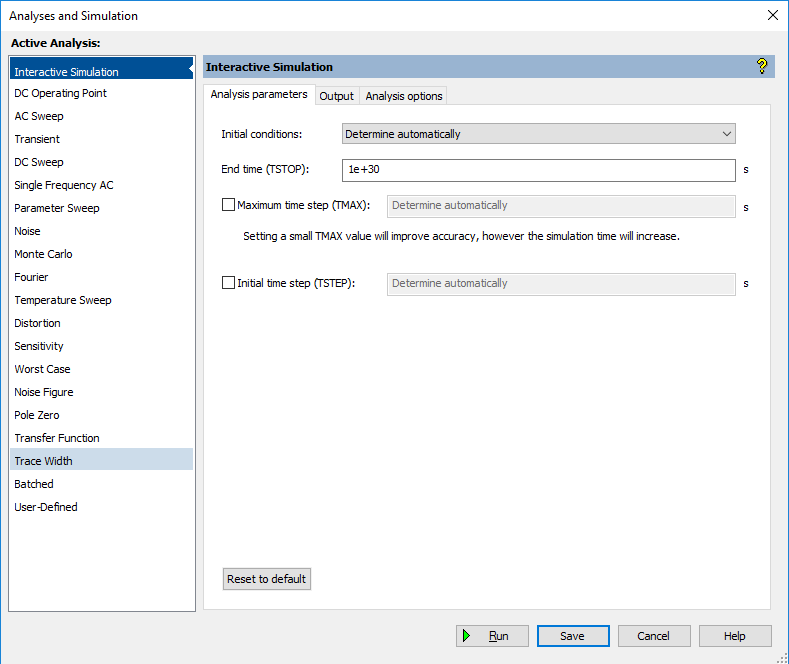
\includegraphics[width=0.55\linewidth]{part4-c-DcOperatingSweep.png}
		\captionof{figure}{The Interactive Simulation Settings of the Test Circuit}\label{f25}
	\end{figure}
	
	\noindent As shown in Figure \ref{f26} below, the signal source is set to provide \textbf{1 kHz sinusoid}.
	The AC base current, $I_B$, is set to \textbf{1 $\mu$A RMS} by adjusting the amplitude of the singal generator to \textbf{0.102 $V_{rms}$}.
	\begin{figure}[!ht]
		\centering
		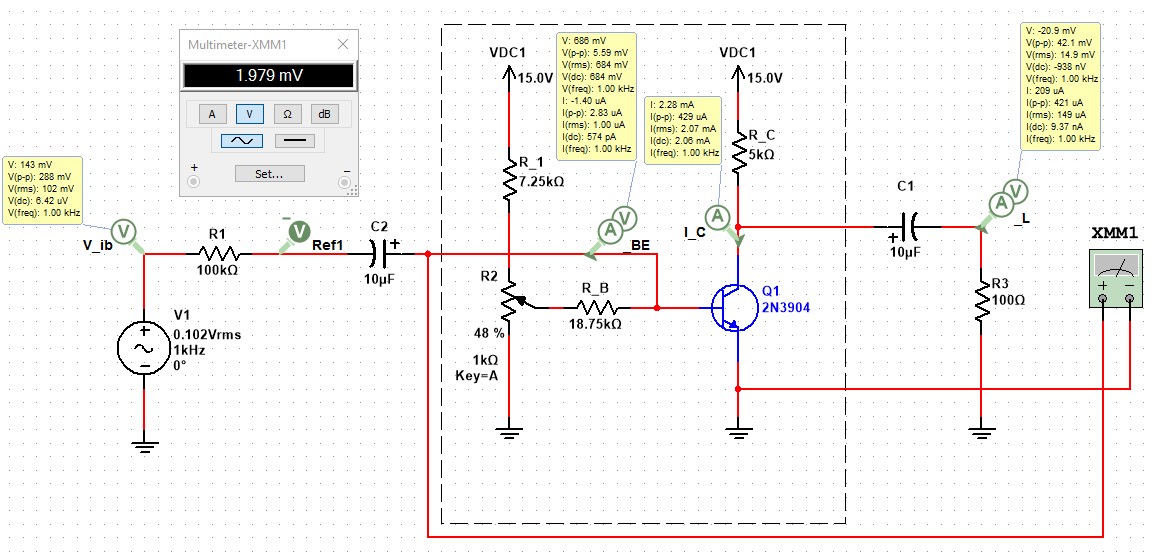
\includegraphics[width=\linewidth]{part4-c-results.png}
		\captionof{figure}{Measured Parameters to Calculate Input Impedance and Current Gain}\label{f26}
	\end{figure}
	
	\noindent \textbf{Note} that all measurements done in this part are RMS.
	
	\pagebreak	
	\noindent\textbf{AC input impedance:}
	\begin{table}[!ht]
		\centering
		\captionof{table}{Measured Parameters to Calculate AC Input Impedance}\label{t7}
		\begin{tabular}{|c|c|c|}
			\hline
			$v_{be}$ & $v_{i_{b}}$ & $R_S$\\
			\hline\hline
			1.976 mV & 100 mV & 100 k$\Omega$\\
			\hline
		\end{tabular}
	\end{table}

	\noindent Using the measured data in Table \ref{t7} above, the AC input impedance is calculated as follows:
	$$h_{ie} = \frac{v_{be}}{i_b} = \frac{v_{be}}{v_{i_{b}}}R_S = \frac{1.976 mV}{100 mV} (100 k\Omega) = 1.976$$
	The AC input impedance is approximately \textbf{2 k$\Omega$}.\\\\
	
	\noindent\textbf{AC forward current gain:}
	\begin{table}[!ht]
		\centering
		\captionof{table}{Measured Parameters to Calculate AC Forward Current Gain}\label{t8}
		\begin{tabular}{|c|c|c|}
			\hline
			$i_b$ & $v_o$ & $R_L$\\
			\hline\hline
			1 $\mu$A & 14.9 mV & 100 $\Omega$\\
			\hline
		\end{tabular}
	\end{table}
	
	\noindent Using the measured data in Table \ref{t8} above, the AC forward current gain is calculated as follows:
	$$h_{fe} = \frac{i_c}{i_b} = \frac{v_o}{R_L * i_b} = \frac{14.9mV}{100\Omega * 1\mu A} = 149$$
	The AC forward current gain is \textbf{149 \textit{A/A}}.\\\\
	A load resistance value of zero is effectively grounding the transistor's collector during AC analysis.
	The load resistor, $R_L$, must be present in the circuit since the AC current and AC voltage of a purely resistive impedance are in phase.
	Regarding that, the output current, $I_{L}$, can be directly calculated using Ohm's law wihtout accounting for phase differences.
	
	
	\pagebreak
	
	\subsubsection{The AC Output Admittance, $h_{oe}$, and the AC Reverse, or Feedback, Voltage Ratio, $h_{re}$}
	From Figure \ref{f9} above, the slope of the $I_C$ vs. $V_{CE}$ characteristics curve is 0.0228 mA/V.
	Therefore, the AC output admittance, $h_{oe}$, is \textbf{22.8 $\mu$mhos}.
	
	\subsubsection{The Unity-Gain Bandwidth, $f_T$, and The Beta Cut-Off Frequency, $f_{\beta}$}
	Figure \ref{f27} below illustrates the test circuit, for $I_C = 2$ mA, and the simulation probes used in this part of the experiment.
	
	\begin{figure}[!ht]
		\centering
		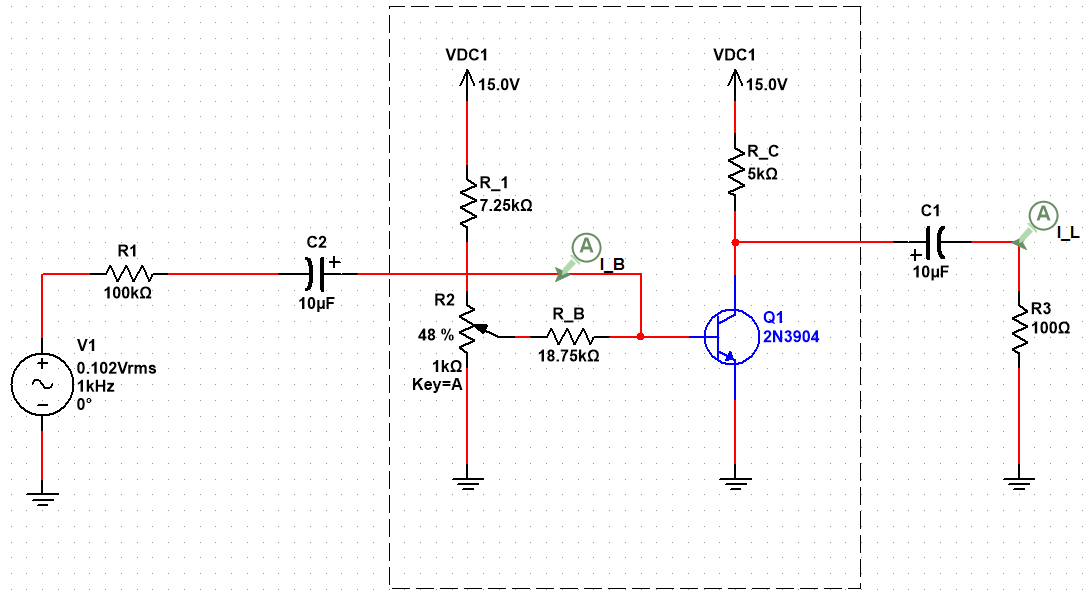
\includegraphics[width=0.8\linewidth]{part4-e-circuit-2ma.png}
		\captionof{figure}{The Test Circuit for The Current Gain for $I_C = 2$ mA}\label{f27}
	\end{figure}

	\noindent Figure \ref{f28} below illustrates the AC sweep settings of the test circuit used in this part of the experiment.
	
	\begin{figure}[!ht]
		\centering
		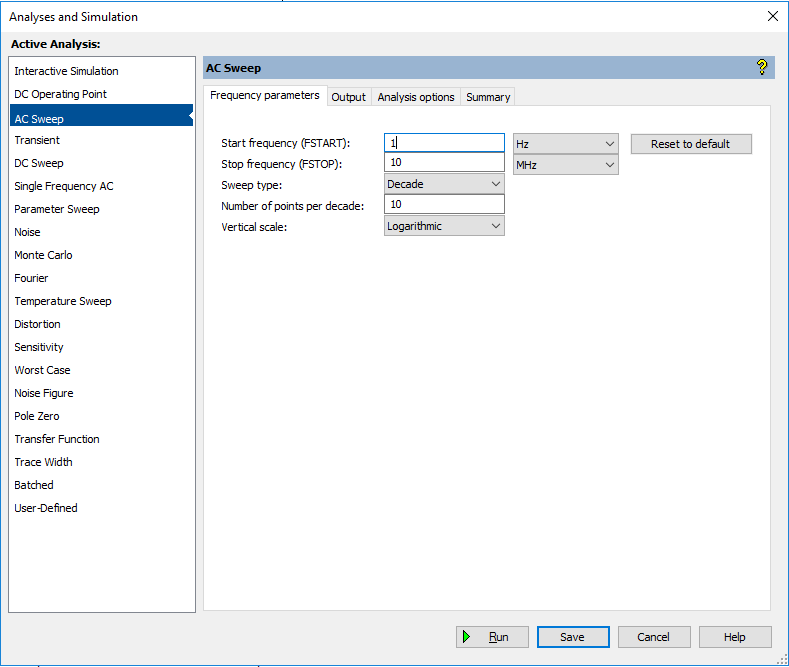
\includegraphics[width=0.6\linewidth]{part4-e-simSettings-2ma.png}
		\captionof{figure}{AC Sweep Simulation Settings for $I_C = 2$ mA}\label{f28}
	\end{figure}
	
	\pagebreak
	
	\begin{table}[!ht]
		\centering
		\captionof{table}{Measured Data to Calculate The Current Gain with $I_C$ = 2 mA}\label{t9}
		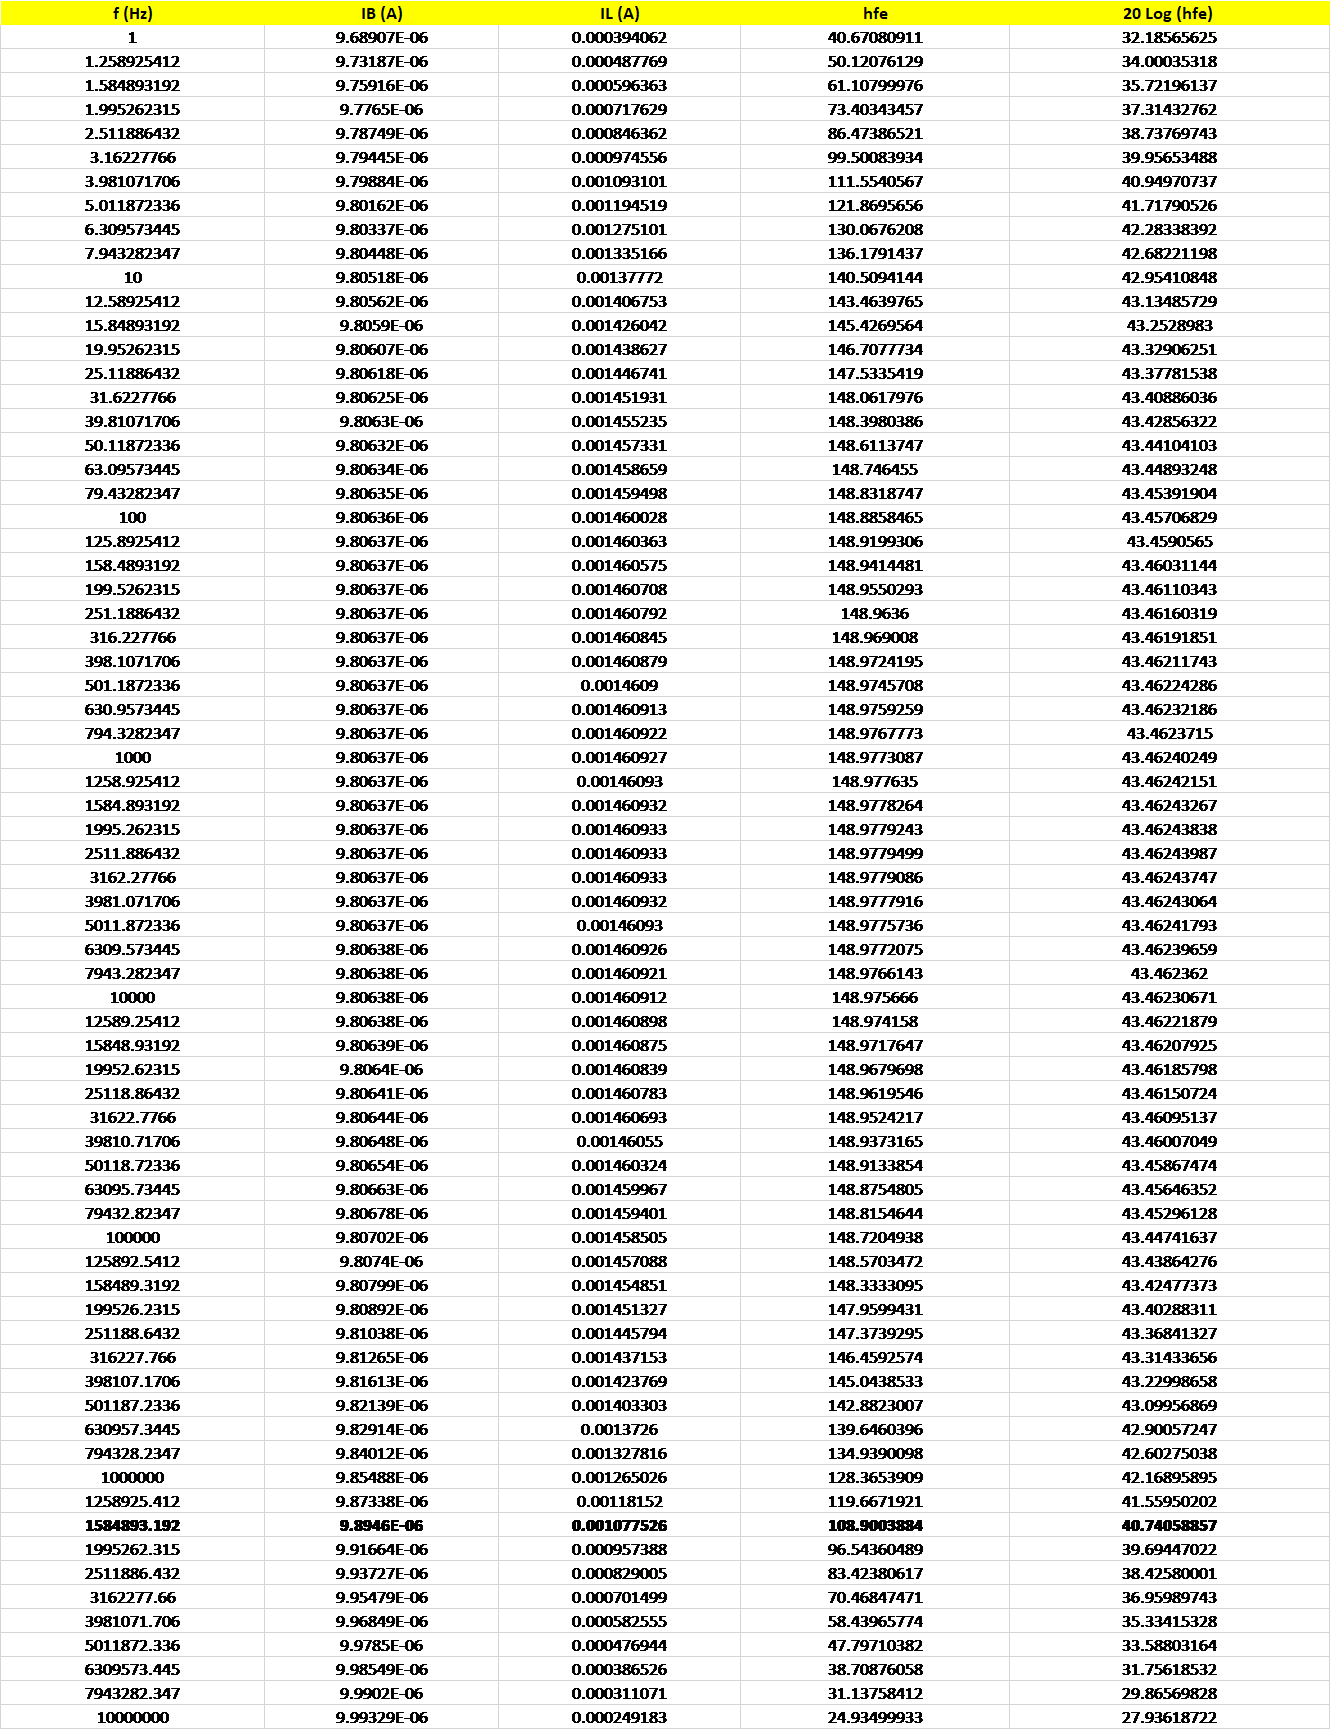
\includegraphics[width=\linewidth]{part4-e-data-2ma.png}	
	\end{table}
	
	\pagebreak
	
	\begin{figure}[!ht]
		\centering
		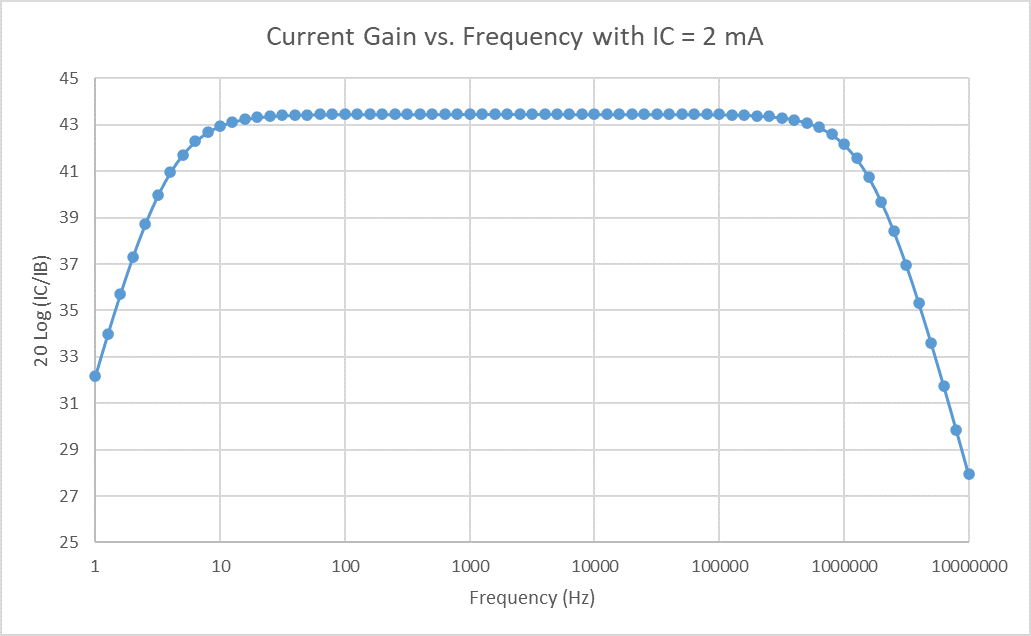
\includegraphics[width=0.6\linewidth]{part4-currentGain-2ma.png}
		\captionof{figure}{Frequency vs. Current Gain with $I_C$ = 2 mA}\label{f29}
	\end{figure}
	
	\begin{table}[!ht]
		\centering
		\captionof{table}{Measured and Calculated Parameters to Unity Gain Bandwidth}\label{t10}
		\begin{tabular}{|c|c|}
			\hline
			$h_{fe_{avg}}$ & $f_{\beta}$\\
			\hline\hline
			148.53 & 1.58 MHz\\
			\hline
		\end{tabular}
	\end{table}	
	
	\noindent Using the measured data in Table \ref{t10} above, the unity-gain bandwidth is calculated as follows:
	$$f_T = h_{fe} * f_{\beta} = (148.53)(1.58 MHz) = 233.84$$
	The Unity-Gain Bandwidth, $f_T$, is equal \textbf{233.84 MHz} when $I_C = 2$ mA.
	
	\pagebreak
	
	\noindent Figure \ref{f30} below illustrates the test circuit, for $I_C = 0.50$ mA, and the simulation probes used in this part of the experiment.
	\begin{figure}[!ht]
		\centering
		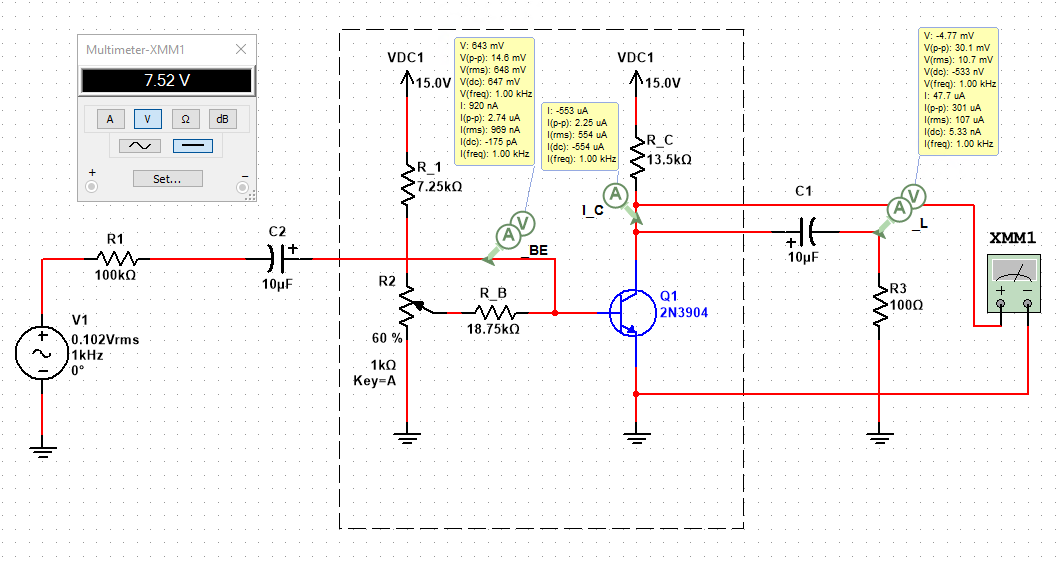
\includegraphics[width=\linewidth]{part4-e-circuit-0.5ma.png}
		\captionof{figure}{The Test Circuit for The Current Gain for $I_C = 0.50$ mA}\label{f30}
	\end{figure}
	
	\noindent Figure \ref{f31} below illustrates the AC sweep settings of the test circuit used in this part of the experiment.
	\begin{figure}[!ht]
		\centering
		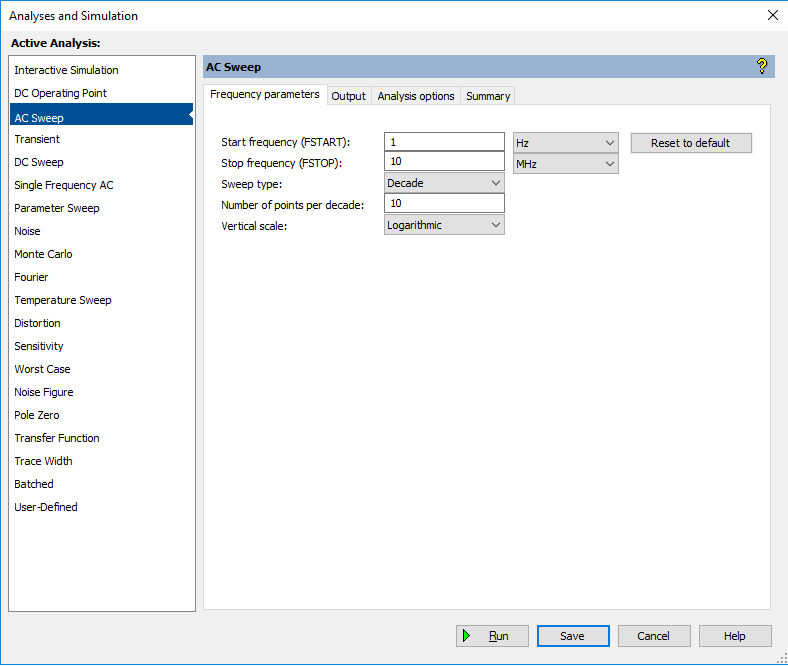
\includegraphics[width=0.7\linewidth]{part4-e-simSettings-0.5ma.png}
		\captionof{figure}{AC Sweep Simulation Settings for $I_C = 0.50$ mA}\label{f31}
	\end{figure}
	
	\pagebreak
	
	\begin{table}[!ht]
		\centering
		\captionof{table}{Measured Data to Calculate The Current Gain with $I_C$ = 0.5 mA}\label{t11}
		\includegraphics[width=\linewidth]{part4-e-data-0.5ma.png}	
	\end{table}
	
	\pagebreak
	
	\begin{figure}[!ht]
		\centering
		\includegraphics[width=0.6\linewidth]{part4-currentGain-0.5ma.png}
		\captionof{figure}{Frequency vs. Current Gain with $I_C$ = 0.5 mA}\label{f32}
	\end{figure}
	
	\noindent As shown in Figure \ref{f30} above, the collector resistor ($R_C$) was set to \textbf{13.5 k$\Omega$} to maintain a collector-emitter voltage ($V_{CE}$) of approximately 7.5 volts.\\\\
	Then, the potentiometer percentage was adjusted to 60\% so that the collector current ($I_C$) is set to approximately 0.5 mA.\\\\
	As shown in Figure \ref{f30} above, the actual collector-emitter voltage ($V_{CE}$) was measured and found to be \textbf{7.52 volts}.
	
	\begin{table}[!ht]
		\centering
		\captionof{table}{Measured and Calculated Parameters to Unity Gain Bandwidth}\label{t12}
		\begin{tabular}{|c|c|}
			\hline
			$h_{fe_{avg}}$ & $f_{\beta}$\\
			\hline\hline
			110.30 & 1.58 MHz\\
			\hline
		\end{tabular}
	\end{table}	
	
	\noindent Using the measured data in Table \ref{t12} above, the unity-gain bandwidth is calculated as follows:
	$$f_T = h_{fe} * f_{\beta} = (110.30)(1.58 MHz) = 174.27$$
	The Unity-Gain Bandwidth, $f_T$, is equal \textbf{174.27 MHz} when $I_C = 0.5$ mA.	
	
	\pagebreak
	
	\noindent Figure \ref{f33} below illustrates the test circuit, for $I_C = 1$ mA, and the simulation probes used in this part of the experiment.
	\begin{figure}[!ht]
		\centering
		\includegraphics[width=\linewidth]{part4-e-circuit-1ma.png}
		\captionof{figure}{The Test Circuit for The Current Gain for $I_C = 1$ mA}\label{f33}
	\end{figure}

	Figure \ref{f34} below illustrates the AC sweep settings of the test circuit used in this part of the experiment.
	\begin{figure}[!ht]
		\centering
		\includegraphics[width=0.7\linewidth]{part4-e-simSettings-1ma.png}
		\captionof{figure}{AC Sweep Simulation Settings for $I_C = 1$ mA}\label{f34}
	\end{figure}

	\pagebreak

	\begin{table}[!ht]
		\centering
		\captionof{table}{Measured Data to Calculate The Current Gain with $I_C$ = 1 mA}\label{t13}
		\includegraphics[width=\linewidth]{part4-e-data-1ma.png}	
	\end{table}
	
	\pagebreak

	\begin{figure}[!ht]
	\centering
	\includegraphics[width=0.6\linewidth]{part4-currentGain-1ma.png}
	\captionof{figure}{Frequency vs. Current Gain with $I_C$ = 0.5 mA}\label{f35}
	\end{figure}

	\noindent As shown in Figure \ref{f33} above, the collector resistor ($R_C$) was set to \textbf{7.25 k$\Omega$} to maintain a collector-emitter voltage ($V_{CE}$) of approximately 7.5 volts.\\\\
	Then, the potentiometer percentage was adjusted to 56\% so that the collector current ($I_C$) is set to approximately 1 mA.\\\\
	As shown in Figure \ref{f33} above, the actual collector-emitter voltage ($V_{CE}$) was measured and found to be \textbf{7.577 volts}.
	
	\begin{table}[!ht]
		\centering
		\captionof{table}{Measured and Calculated Parameters to Unity Gain Bandwidth}\label{t14}
		\begin{tabular}{|c|c|}
			\hline
			$h_{fe_{avg}}$ & $f_{\beta}$\\
			\hline\hline
			132.53 & 1.58 MHz\\
			\hline
		\end{tabular}
	\end{table}	

	\noindent Using the measured data in Table \ref{t14} above, the unity-gain bandwidth is calculated as follows:
	$$f_T = h_{fe} * f_{\beta} = (132.53)(1.58 MHz) = 209.39$$
	The Unity-Gain Bandwidth, $f_T$, is equal \textbf{209.39 MHz} when $I_C = 1$ mA.

	\pagebreak
	
	\subsection{The BJT High-Frequency Hybrid-Pi Model}
	Figure \ref{f36} below shows the high-frequency hybrid-pi model of a BJT.
	\begin{figure}[!ht]
		\centering
		\includegraphics[width=0.75\linewidth]{hybridpi.png}
		\captionof{figure}{The High-Frequency Hybrid-Pi Model of a BJT}\label{f36}
	\end{figure}
	
	\noindent The equations below define its elemental values in terms of the previously measured circuit parameters.
	
	\pagebreak
	
	\subsubsection{Calculations given $I_C$ = 2 mA}
	\vspace{0.5cm}
	$$g_m = \frac{I_C}{V_T} = \frac{2mA}{25mV} = 80 \hspace{1mm} milli \hspace{1mm} mhos$$
	$$r_{\pi} = \frac{h_{fe}}{g_m} = \frac{148.53}{0.08} = 1.856 k\Omega$$
	$$r_x = h_{ie} - r_{\pi} = 1.976 k\Omega - 1.856 k\Omega = 120\Omega$$
	$$r_{\mu} = \frac{r_{\pi}}{h_{re}} \approx \infty$$
	$$r_o = (h_{oe} - \frac{h_{fe}}{r_{\mu}})^{-1} \approx {h_{oe}}^{-1} \approx (22.8 \hspace{1mm} \mu mhos)^{-1} \approx 44 k\Omega$$
	$$\omega_{\beta} = 2\pi f_{\beta} = (2\pi) (1.58 MHz) = 9.93 \hspace{1mm} Mrad/sec$$
	$$C_{\mu} = C_{BC_{junction}} + C_{board} \approx 2pf + 2pf = 4pf$$
	$$C_{\pi} = \frac{1}{r_{\pi} * \omega_{\beta}} - C_{\mu} \left [ 1 + \left | \frac{v_o}{v_{be}} \right |_{@ 1kHz} \right ] = \frac{1}{(1.856 k\Omega) (9.93 \hspace{1mm} Mrad/sec)} - (4pf) \left [ 1 + \left | \frac{1.02 \mu V}{684mV} \right |_{@ 1kHz} \right ] \approx 50pf$$
	
	\pagebreak
	
	\subsubsection{Calculations given $I_C$ = 0.5 mA}
	\vspace{0.5cm}
	$$g_m = \frac{I_C}{V_T} = \frac{0.5mA}{25mV} = 20 \hspace{1mm} milli \hspace{1mm} mhos$$
	$$r_{\pi} = \frac{h_{fe}}{g_m} = \frac{110.30}{0.02} = 5.515 k\Omega$$
	$$r_x = h_{ie} - r_{\pi} = 1.976 k\Omega - 5.515 k\Omega = - 3.539 k\Omega \approx 0$$
	$$r_{\mu} = \frac{r_{\pi}}{h_{re}} \approx \infty$$
	$$r_o = (h_{oe} - \frac{h_{fe}}{r_{\mu}})^{-1} \approx {h_{oe}}^{-1} \approx (22.8 \hspace{1mm} \mu mhos)^{-1} \approx 44 k\Omega$$
	$$\omega_{\beta} = 2\pi f_{\beta} = (2\pi) (1.58 MHz) = 9.93 \hspace{1mm} Mrad/sec$$
	$$C_{\mu} = C_{BC_{junction}} + C_{board} \approx 2pf + 2pf = 4pf$$
	$$C_{\pi} = \frac{1}{r_{\pi} * \omega_{\beta}} - C_{\mu} \left [ 1 + \left | \frac{v_o}{v_{be}} \right |_{@ 1kHz} \right ] = \frac{1}{(1.856 k\Omega) (9.93 \hspace{1mm} Mrad/sec)} - (4pf) \left [ 1 + \left | \frac{533nV}{647mV} \right |_{@ 1kHz} \right ] \approx 50pf$$
	
	\pagebreak
	\subsubsection{Calculations given $I_C$ = 1 mA}
	\vspace{0.5cm}
	$$g_m = \frac{I_C}{V_T} = \frac{1mA}{25mV} = 40 \hspace{1mm} milli \hspace{1mm} mhos$$
	$$r_{\pi} = \frac{h_{fe}}{g_m} = \frac{132.53}{0.04} = 3.313 k\Omega$$
	$$r_x = h_{ie} - r_{\pi} = 1.976 k\Omega - 3.313 k\Omega = - 1.337 k\Omega \approx 0$$
	$$r_{\mu} = \frac{r_{\pi}}{h_{re}} \approx \infty$$
	$$r_o = (h_{oe} - \frac{h_{fe}}{r_{\mu}})^{-1} \approx {h_{oe}}^{-1} \approx (22.8 \hspace{1mm} \mu mhos)^{-1} \approx 44 k\Omega$$
	$$\omega_{\beta} = 2\pi f_{\beta} = (2\pi) (1.58 MHz) = 9.93 \hspace{1mm} Mrad/sec$$
	$$C_{\mu} = C_{BC_{junction}} + C_{board} \approx 2pf + 2pf = 4pf$$
	$$C_{\pi} = \frac{1}{r_{\pi} * \omega_{\beta}} - C_{\mu} \left [ 1 + \left | \frac{v_o}{v_{be}} \right |_{@ 1kHz} \right ] = \frac{1}{(1.856 k\Omega) (9.93 \hspace{1mm} Mrad/sec)} - (4pf) \left [ 1 + \left | \frac{4.31 \mu V}{664mV} \right |_{@ 1kHz} \right ] \approx 50pf$$
	
	\pagebreak
	
	\section{Conclusion}
	In conclusion, a full DC and AC analysis was performed for several different BJT circuits.
	After discovering that the 2N3904 transistor is an NPN BJT type and the 2N3906 transistor is a PNP BJT type, the DC output characteristics were found for the NPN BJT.
	It was seen that $V_{BE}$ remains constant while $V_{CE}$ increases (only when BJT is operating in the active region).
	Once the BJT enters the saturation mode, $V_{BE}$ starts to slowly decrease.\\\\
	Two NPN BJTs were used to create both a 1:1 and 1:2 current mirror, which could be used as a current source.
	It was observed that the amplified output current (in the case of the 1:2 current mirror) did not change drastically in value for all load resistance values that kept the BJT in the active mode.
	This circuit will be useful in the future as a current source, as different circuits with varying “load resistances” will connect to it (while receiving the same current input).\\\\
	A full AC analysis was performed on the BJT by attaching an AC source using capacitors.
	The capacitors blocked all DC signals, so a detailed AC analysis was possible to achieve.
	Many small signal model parameters were derived and calculated.\\\\
	Finally, the values obtained in Part 4 were used to calculate the remaining small signal parameters, including $g_m$ and $C_{\pi}$.
	The value of $C_{\pi}$ was found to be 50pf, which will be useful in the future for the design of an amplifier circuit.
	
	\pagebreak
	
	\section{References}
	[1] “Lab 1: The Bipolar Junction Transistor (BJT): DC and AC Characterization,” Carleton Univeristy, Ottawa, 2017.
\end{document}